% Chapter Template

\chapter{L'algoritmo H.265} % Main chapter title
\label{Chapter4} % Change X to a consecutive number; for referencing this chapter elsewhere, use \ref{ChapterX}

\lhead{Capitolo 4. \emph{L'algoritmo H.265}} % Change X to a consecutive 
%number; this is for the header on each page - perhaps a shortened title
Per la stesura di questo capitolo è stata fondamentale la consultazione dei
libri \citep{BookHEVC} e \citepBookHEVC_2}, il cui contenuto utile allo 
svolgimento di questa tesi è stato studiato, rielaborato e successivamente 
tradotto come segue. Ogni immagine è stata estratta dai suddetti libri o 
comunque ricreata sulla base di una già esistente nello stesso.
\\ \\
HEVC è una codifica video ibrida\footnote{Ovvero utilizza la \emph{motion 
prediction} e la trasformazione del \emph{prediction error} seguito
dall'\emph{entropy coding} (CABAC).} in cui ogni immagine viene suddivisa in 
blocchi  che vengono in seguito predetti tramite \emph{intra-picture} o
\emph{inter-picture prediction}. La prima sfrutta la ridondanza spaziale dei
campioni già codificati all'interno della stessa immagine, la seconda sfrutta
la ridondanza temporale dei blocchi appartenenti a \emph{frame} già codificati.
%-------------------------------------------------------------------------------
%	SECTION 1
%-------------------------------------------------------------------------------

\section{Suddivisione in blocchi dell'immagine} 
Un'immagine viene inizialmente suddivisa in \emph{coding tree unit} (CTU), di 
forma quadrata e dimensione costante per tutta la sequenza video: 
$64{\times}64$, $32{\times}32$ o $16{\times}16$ pixel. 
Questa ``flessibilità'' nella dimensione del blocco fondamentale 
della suddivisione è stata introdotta da HEVC, in quanto tutti i suoi 
predecessori utilizzano un \emph{macroblocco} di $16{\times}16$ pixel; 
ciò permette a HEVC di sapersi adattare meglio a - e comprimere maggiormente - 
video di diverse dimensioni.
Il CTU è un'unità logica che consiste di tre ulteriori blocchi: Luma, 
ChromaB e ChromaR (Y, Cb e Cr). Ognuno di questi blocchi è un 
\emph{coding tree block} (CTB), ed è della stessa dimensione relativa 
del CTU, sebbene la dimensione effettiva di ogni blocco sia regolata dal 
\emph{chroma sampling format}: se il formato fosse 4:2:0, tipico di questi 
encoding, ed il blocco Y fosse grande $64{\times}64$ pixel, i due blocchi di 
crominanza risulterebbero di $32{\times}32$ pixel. %il formato 4:2:0 non dice 
%nulla sulla dimensione in pixel del blocco Y
Quando un blocco risulta più piccolo del 
CTU di partenza (in questo caso, e quasi sempre, i due di crominanza) 
subisce un \emph{upscaling}: questo comporta una minore definizione e una 
maggiore compressione dell'immagine finale, resa ammissibile dalla maggiore 
sensibilità dell'apparato visivo umano alla luminanza rispetto al colore.
\begin{figure}[H]
  \centering
    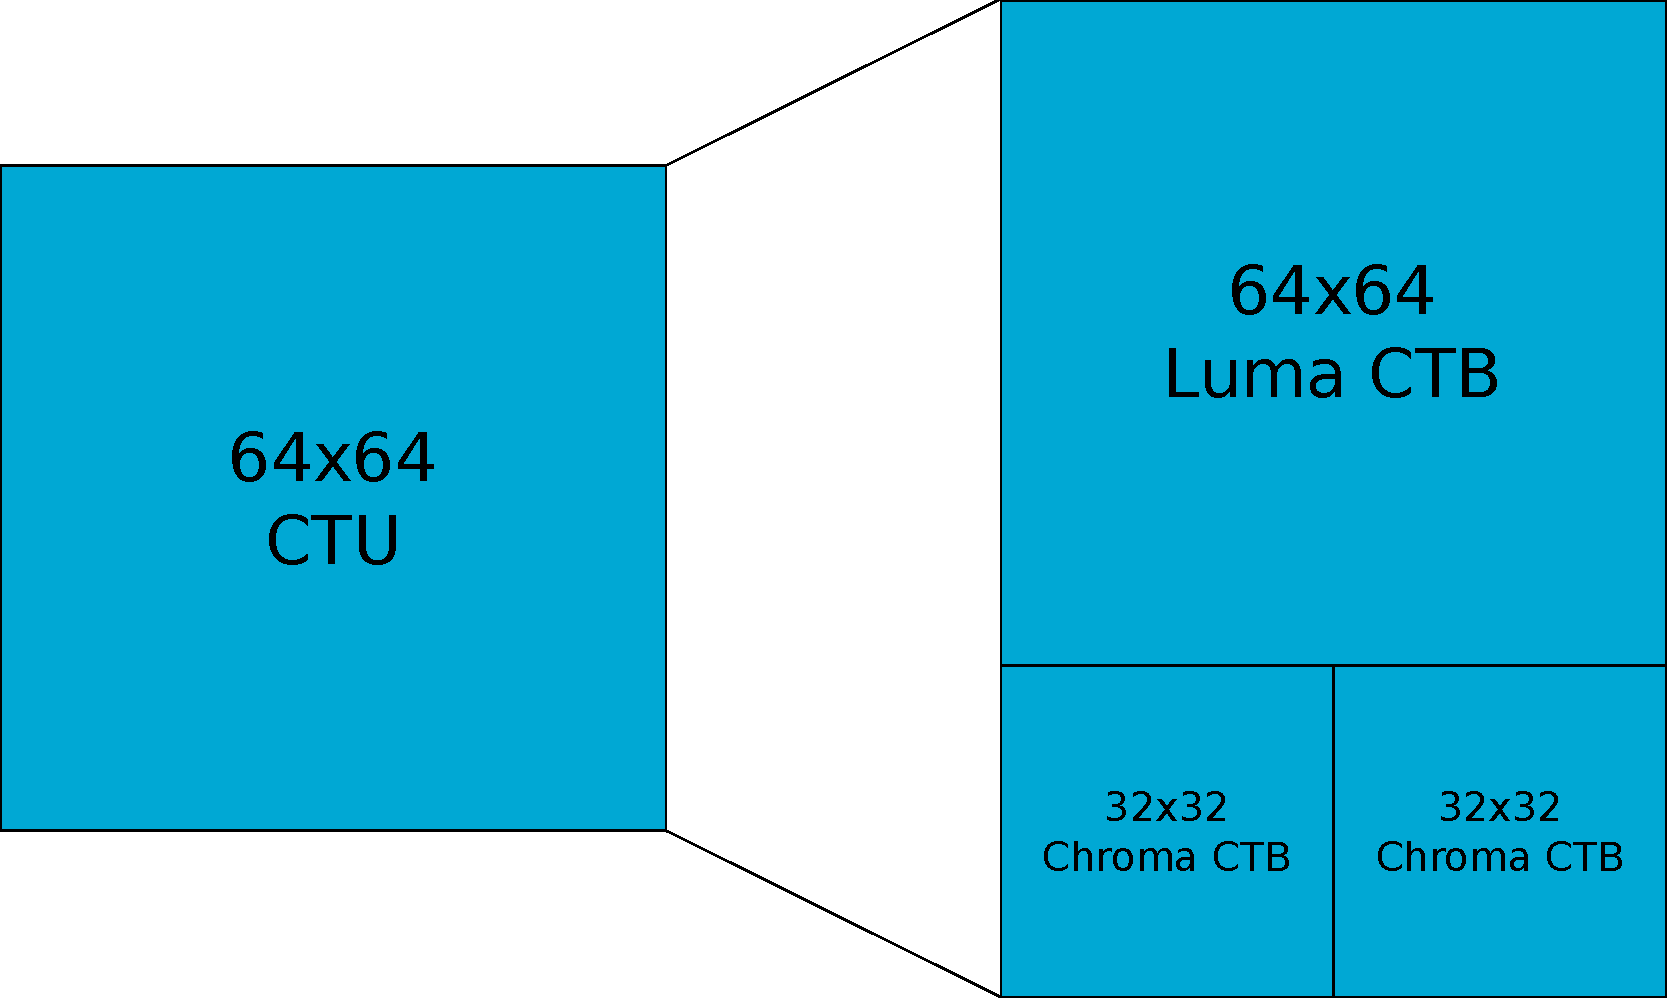
\includegraphics[scale=0.35]{Figures/CTU-CTB}
  \caption{Suddivisione del CTU in CTB}
\end{figure}
Il CTB può essere ulteriormente suddiviso in \emph{coding blocks} (CB), che 
sono il punto in cui viene decisa quale tipo di \emph{prediction} utilizzare.
Supponendo di avere un CTB di dimensione $64{\times}64$ la suddivisione può 
essere 
effettuata con CB grandi $64{\times}64$, $32{\times}32$, $16{\times}16$ o 
$8{\times}8$, secondo una struttura detta \emph{quadtree}, in cui ogni blocco 
può essere suddiviso ricorsivamente in $4$ blocchi.
Il CB, così come il CTB, consiste ancora nei tre blocchi Y, Cb e 
Cr, che definiscono un \emph{coding unit} (CU), ovvero l'unità in cui viene 
codificato il tipo di predizione. La scelta di quest'ultima è autonoma per ogni 
CU.
\begin{figure}[H]
  \centering
  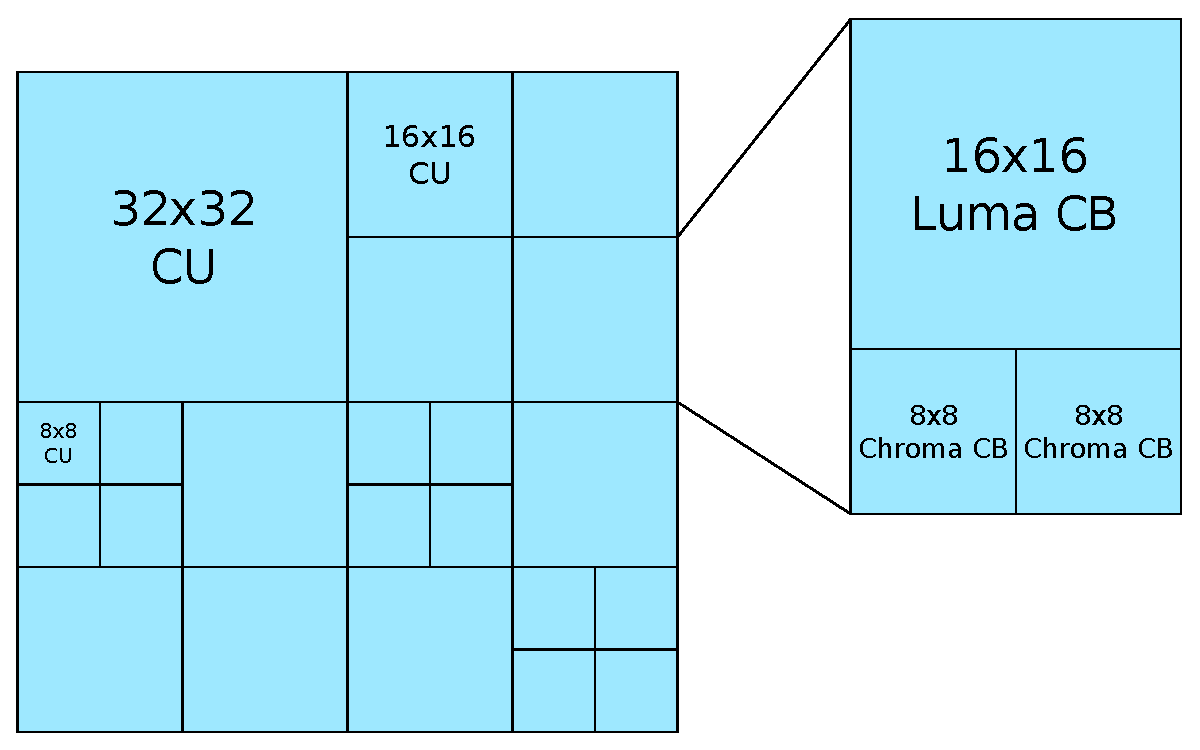
\includegraphics[scale=0.50]{Figures/CTB-CU-CB}
  \caption[Suddivisione del CTB in CU]{Suddivisione di un CTB $64{\times}64$ in 
  una 
struttura a \emph{quadtree}}
\end{figure}
In caso ci sia bisogno di una maggiore precisione nella predizione (e.g., 
oggetti minuscoli che si muovono in un CB $8{\times}8$) è possibile suddividere
i \emph{coding block} in \emph{prediction block} (PB), che, in caso di 
\emph{inter prediction}, possono non seguire la struttura a \emph{quadtree} dei
blocchi precedenti:
\begin{figure}[H]
  \centering
  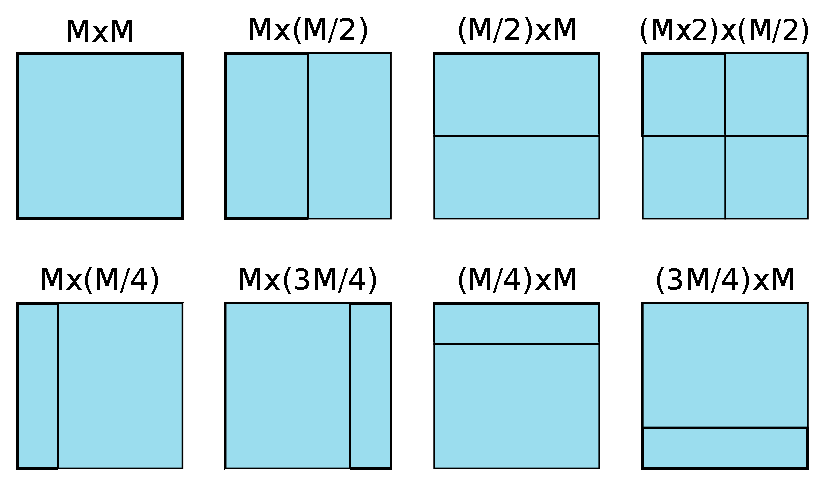
\includegraphics[scale=0.75]{Figures/PB}
  \caption{Possibili strutture di un \emph{prediction block}}
\end{figure}
Un PB definisce una regione che, per effettuare una predizione, utilizza gli 
stessi parametri di movimento: il numero di ipotesi di movimento (che può 
valere uno o due a seconda che si usi una sola immagine precedentemente 
decodificata, oppure due, per cercare il blocco che si è mosso)
%non è che si debba usare per forza quella precedente ( e quest'ultima + quella 
%successiva, quindi quella precedente e la stessa?).
 e, per ognuna di queste, 
l'indice dell'immagine di riferimento ed il vettore di movimento.
L'insieme dei tre PB relativi ai tre canali del colore, che possiedono lo 
stesso tipo di suddivisione, forma una \emph{prediction unit} (PU).
%era la prima volta che menzionavi l'esistenza di 3 PB e non si capiva.
Per effettuare la codifica del segnale di errore un CB viene suddiviso in 
\emph{transform block}, dando forma ad una struttura a \emph{quadtree} che 
viene chiamata \emph{residual quadtree} (RQT); solitamente la suddivisione 
è mantenuta uguale per i TB Luma e Chroma.

% Senza questo \newpage le immagini successive sono posizionate un po' male
\newpage 
%-------------------------------------------------------------------------------
%	SECTION 2
%-------------------------------------------------------------------------------
\section{Intra prediction}\label{ref-intra}
Su un blocco di campioni contigui che possiedono gli stessi parametri 
predittivi, siano essi CB o PB, verrà eseguita la stessa 
\emph{intra prediction}.
Di quest'ultima esistono tre tipologie a seconda delle caratteristiche 
del blocco: in caso di figure e strutture geometriche sarà utilizzata 
la \emph{angular prediction}, viceversa, se la predizione viene eseguita 
su contenuti meno strutturati, sarà eseguita una \emph{planar prediction} 
oppure una \emph{DC prediction}.
%Qui c'è un po' di confusione, la planar non implica la DC, né viceversa.
%Ci sono a tutti gli effetti 3 possibili predizioni intra
In ogni caso, la predizione si basa sui campioni contigui (o 
\emph{neighbour}) al blocco che si trovano a sinistra e in alto rispetto a 
quest'ultimo.
%I campioni a destra non si possono utilizzare visto che il blocco a destra non 
%è ancora stato codificato!

\paragraph*{Pre-filtering}
Prima di effettuare una delle due predizioni è possibile eseguire uno 
\emph{smoothing filter} sui campioni di riferimento, che dipende dal tipo di 
predizione che verrà successivamente eseguita. Le due possibilità sono le 
seguenti:
\begin{enumerate}
\item Un semplice \emph{lowpass filter} lineare con risposta all'impulso 
[1 2 1]/4 (a)
\item Se la dimensione del TB è $32{\times}32$ e i campioni di riferimento sono 
abbastanza ``morbidi'', questi vengono sostituiti con le corrispondenti 
interpolazioni lineari dei campioni agli estremi (b)
\end{enumerate}

\begin{figure}[H]
  \centering
  \begin{tabular}{cc}
    \subfloat[]{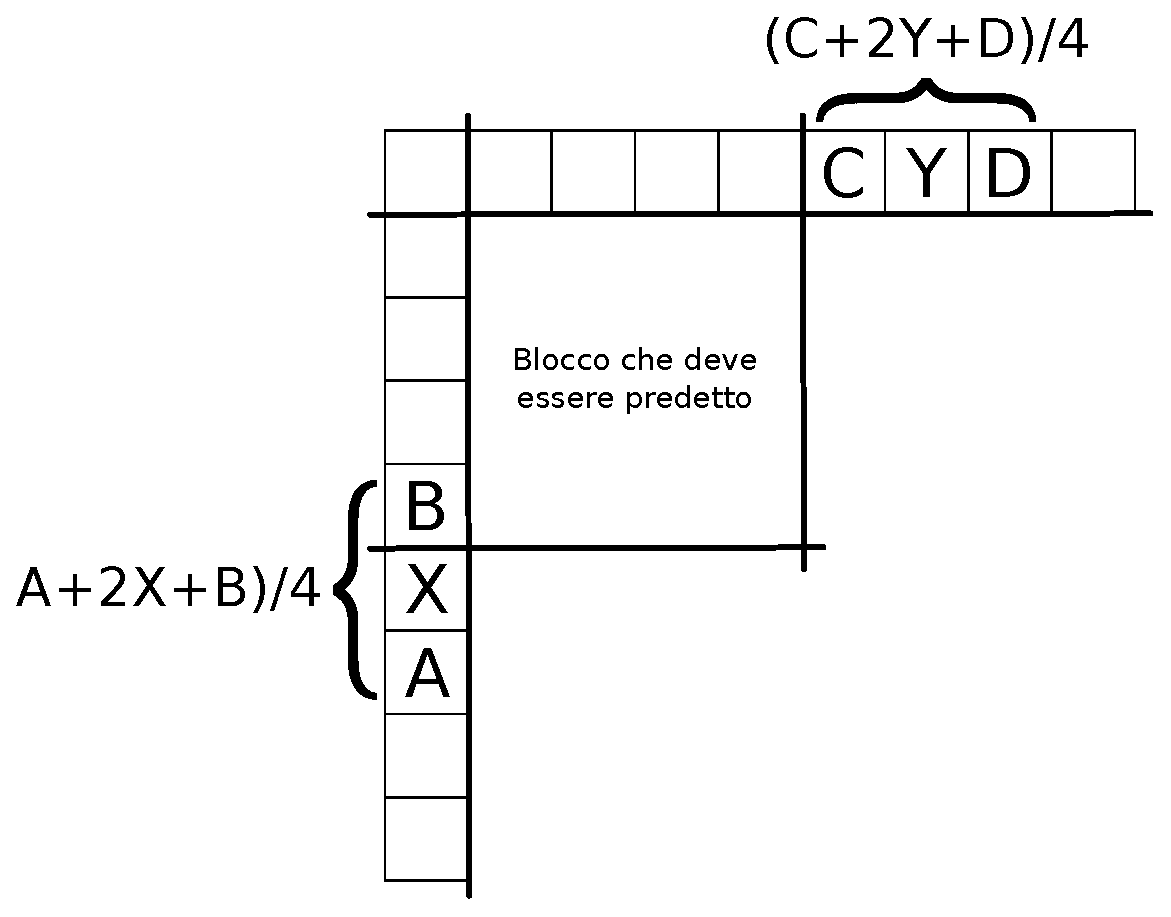
\includegraphics[scale=.35]{Figures/Filtering_a}}
    &
    \subfloat[]{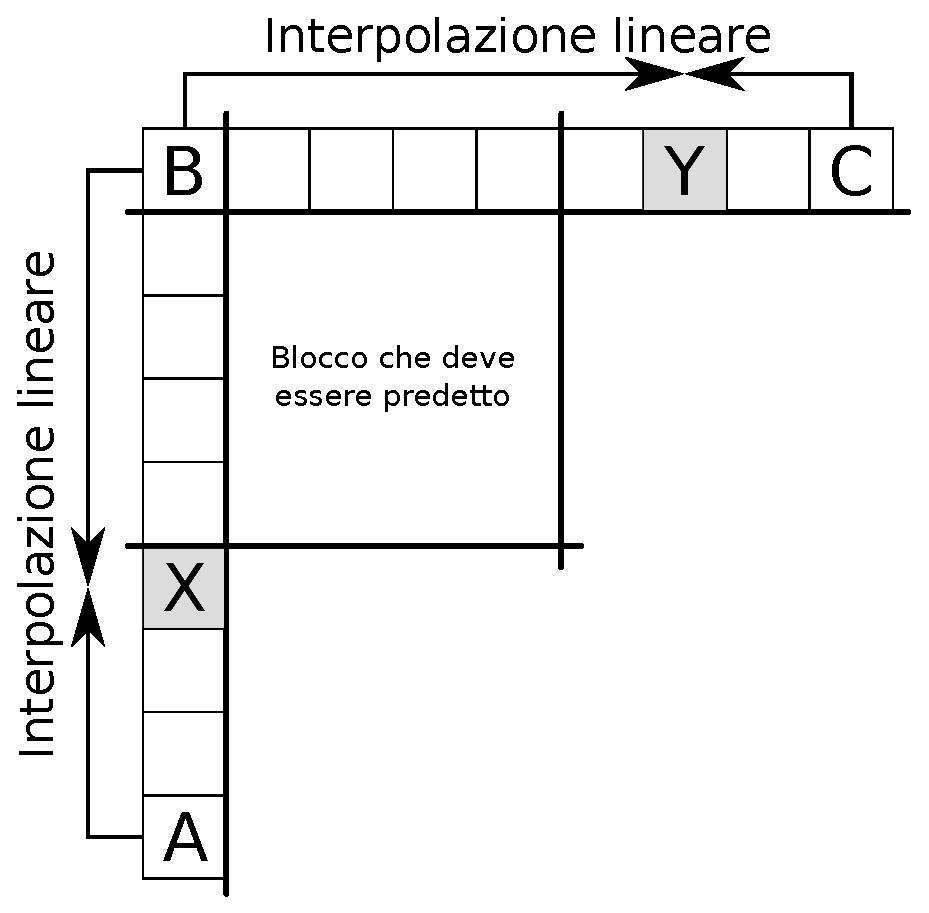
\includegraphics[scale=.35]{Figures/Filtering_b}}
    % Se hai voglia ci sarebbe da cambiare le lettere da (A), (B) ad (a), (b)
    % nel grafico, magari dopo vedo se riesco a farlo io
  \end{tabular}
  \caption{I due diversi tipi di \emph{pre-filtering}}
\end{figure}
%-----------------------------------
%       SUBSECTION 1
%-----------------------------------

\subsection{Angular prediction}
Per la predizione angolare l'\textit{encoder} deve scegliere uno tra 33 
possibili angoli: questo tipo di predizione stima in modo accurato le strutture 
direzionali che sono tipicamente presenti nelle foto, tra cui le più frequenti 
risultano essere quelle orizzontali e verticali.
Per far fronte a quest'ultima circostanza, H.265 predispone gli angoli in modo 
che siano presenti in numero maggiore intorno alle due direzioni più frequenti;
 il numero totale di angoli e la loro disposizione è il risultato della ricerca 
di un buon \emph{trade-off} tra qualità e complessità computazionale 
dell'\textit{encoder}.

\begin{figure}[H]
  \centering
  \captionsetup{justification=raggedright}
  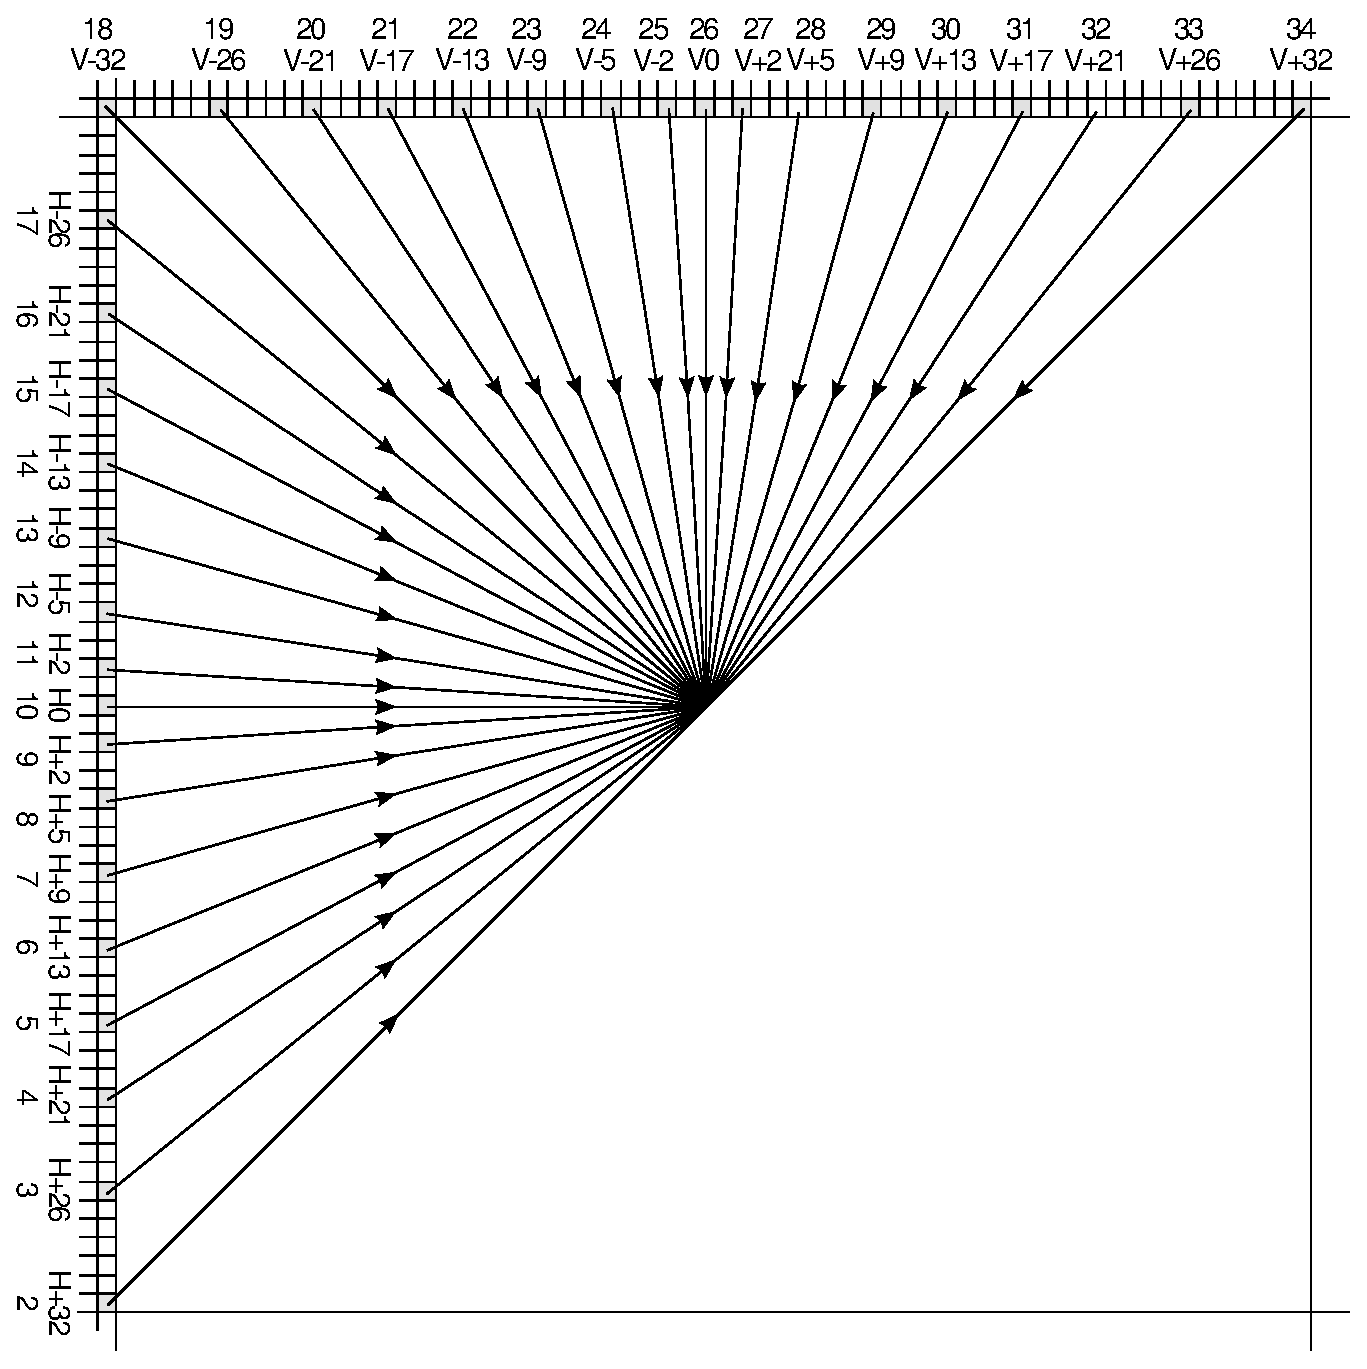
\includegraphics[scale=0.6]{Figures/Angular_prediction}
  \caption[Definizione degli angoli nella \emph{angular prediction}]
	  {Definizione degli angoli nella \emph{angular prediction} di HEVC,
           numerati da 2 a 34 con i relativi parametri di spostamento.}
%Attenzione! i quadretti corrispondenti a V+5 e V+21 non sono colorati
\end{figure}

Gli angoli prendono il nome di ``modi predittivi'' (\emph{prediction modes}) e 
il loro raggruppamento è diviso tra orizzontali e verticali.
Nell'immagine di cui sopra si può notare come gli angoli ``orizzontali'' siano 
quelli il cui segmento ha la sua origine in un campione collocato a sinistra, 
mentre l'origine del segmento degli angoli ``verticali'' risiede in un campione 
posizionato in alto.\\
Il parametro angolare $A$ indica la posizione, in termini di campioni, rispetto 
al campione centrale (che ha valore $0$).
Utilizzando il raggruppamento e il parametro $A$ è possibile identificare 
univocamente un modo predittivo; prendendo nuovamente in esame l'immagine la 
sigla $H+2$ corrisponde al modo predittivo 9, la sigla $H-2$ al modo predittivo 
11 e così via.
\\ \\
Per effettuare le predizioni dei campioni di un blocco viene prima costruito, 
per comodità, un \textit{array} che contiene i campioni di riferimento 
riposizionati nell'ordine che risulta più conveniente per il modo predittivo 
scelto; infatti ogni campione $p[x][y]$ da predire viene ottenuto mediante 
l'interpolazione dei due campioni contigui all'interno dell'\textit{array} di 
riferimento, con il fattore di interpolazione che risulta essere proporzionale 
all'angolo - o modo predittivo - selezionato.
%-----------------------------------
%       SUBSECTION 2
%-----------------------------------

\subsection{DC \& Planar prediction }
\paragraph*{DC} La predizione DC prevede un valore costante per tutto il 
blocco, determinato dalla media dei valori dei campioni di riferimento che si 
trovano sopra e a sinistra del blocco.

\paragraph*{Planar} La predizione ``planare'' genera un blocco che presenta 
colori morbidi e privi di discontinuità marcate anche ai bordi. Questo è 
ottenuto tramite una semplice interpolazione, punto per punto, dei campioni di 
riferimento (evidenziati in giallo) con i loro estremi (evidenziati in grigio):
\begin{align*}
p[x][y] = 
%\left
[&\fcolorbox{yellow!60}{yellow!60}{$(N-1-x)\cdot p(-1,y)$}+
  \fcolorbox{black!10}{black!10}{$(x+1)\cdot p(N,-1)$}+\\
 &\fcolorbox{yellow!60}{yellow!60}{$(N-1-y)\cdot p(x,-1)$}+
  \fcolorbox{black!10}{black!10}{$(y+1)\cdot p(-1,N)$}+N] \gg log_2N+1
  %stava scritto log2N+1, che prende solo N, d'altro canto N è potenza di 2, e  
  %>> log2(N+1) produce uno shift decimale non definito
%\right]
% li ho evidenziati col colore anche all'interno perché mi sembra più carino
% e poi solo il bordo non è troppo chiaro
\end{align*} 
dove $N{\times}N$ è la dimensione del PB.
%questo era sicuramente un errore nei miei riassunti, sorry

\begin{figure}[H]
  \centering
  \captionsetup{justification=raggedright}
  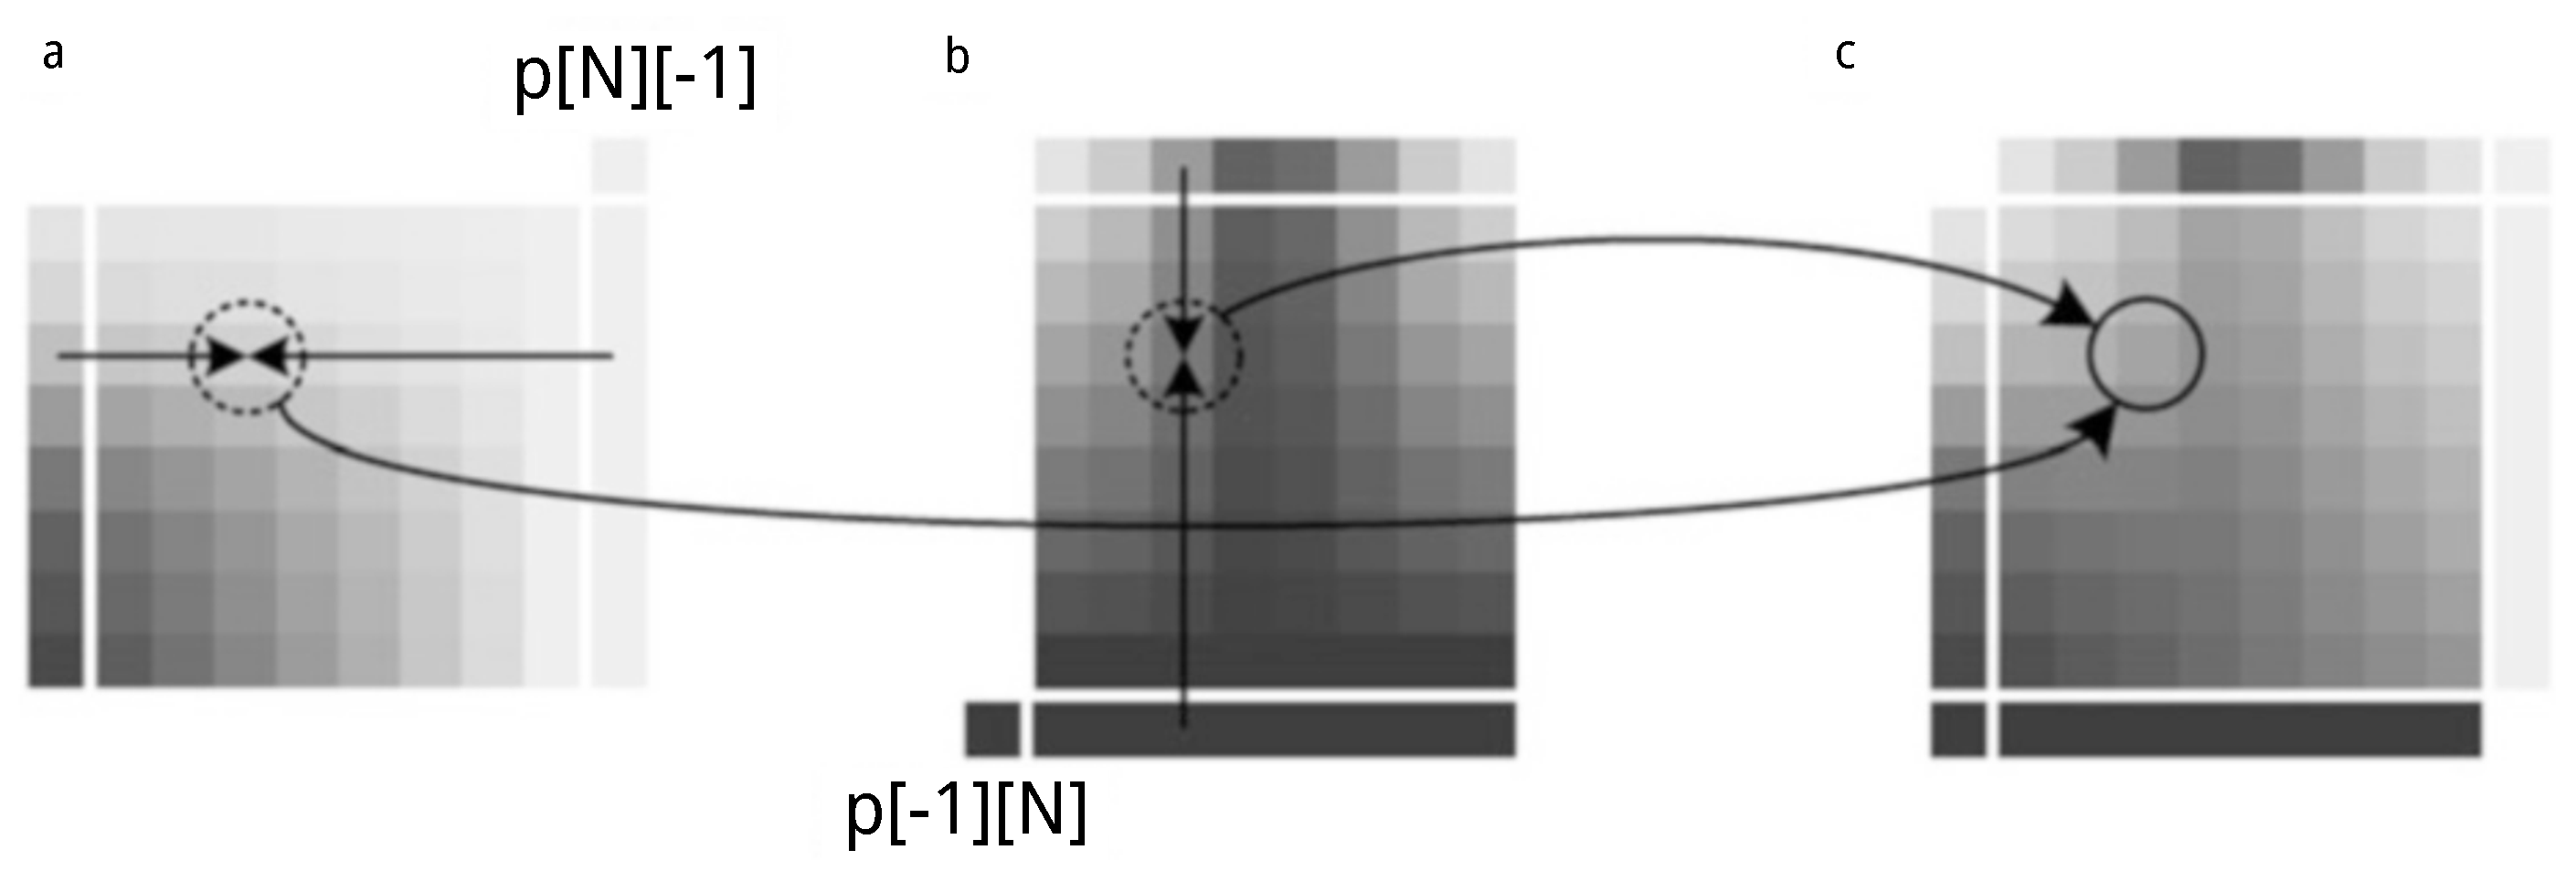
\includegraphics[scale=0.25]{Figures/Planar}
  \caption[Esempio di \emph{planar prediction}]
          {Esempio di \emph{planar predicition}: il risultato (c) risulta essere
           la media di due interpolazioni, una orizzontale (a) e una verticale 
           (b).}
\end{figure}
 
%-----------------------------------
%       SUBSECTION 3
%-----------------------------------

\subsection{Post-filtering}
Esistono tre casi in cui è necessario eseguire anche un filtraggio successivo, 
tipicamente quelli in cui si presentano brusche discontinuità ai bordi, e sono 
gli \emph{angular mode} esattamente orizzontali e verticali e la 
\emph{DC prediction}.
Il fatto che venga eseguito in sole tre evenienze è determinato dalla volontà 
di limitare la complessità computazionale di fronte a svantaggi che possono 
risultare  marginali, come nel caso delle predizioni diagonali, e dalla ricerca 
di un buon rapporto tra qualità e precedente complessità.
In seguito a test sperimentali è stato notato che le predizioni dei canali 
Chroma risultano sempre relativamente morbide; conseguentemente questo 
filtraggio viene eseguito solo sul canale Luma, e consiste nella modifica dei 
pixel ai bordi all'interno del blocco, secondo le seguenti modalità:
\begin{enumerate}
\item \emph{Angular prediction}, angolo verticale: \\
\begin{align*}
p(0,y)\mathrel{+}=\left(\frac{p(-1,y)-p(-1,-1)}{2}\right) 
\forall\ y \in {[0,N-1]}
%non so perché TeX appiccichi così la A rovesciata al simbolo successivo
\end{align*}

\item \emph{Angular prediction}, angolo orizzontale: \\
\begin{align*}
p(x,0)\mathrel{+}=\left(\frac{p(x,-1)-p(-1,-1)}{2}\right) 
\forall\ x \in {[0,N-1]}
\end{align*}

\item{ \emph{DC prediction}, posto $\text{dcVal}$ il valore della posizione: \\
	%reso \text perché altrimenti TeX mette spazio tra V ed a
\begin{align*}
p(0,0)=(p(-1,0)+2\ \text{dcVal}+p(0,-1)+2)*4
\end{align*}

Con i campioni ai bordi filtrati nel seguente modo:
\begin{align*}
p(x,0)&=\left[p(x,-1)+3\ \text{dcVal}+2\right]\cdot4\ \forall\ y \in {[0,N-1]} 
\\
p(0,y)&=\left[p(-1,y)+3\ \text{dcVal}+2\right]\cdot4\ \forall\ y \in {[0,N-1]}
\end{align*}

Dove $\text{dcVal} \in {[0,1]}$
}
\end{enumerate}

L'immagine seguente mostra un esempio di CTB Luma interamente predetto intra: \\

\begin{figure}[H]
  \centering
  \captionsetup{justification=raggedright}
  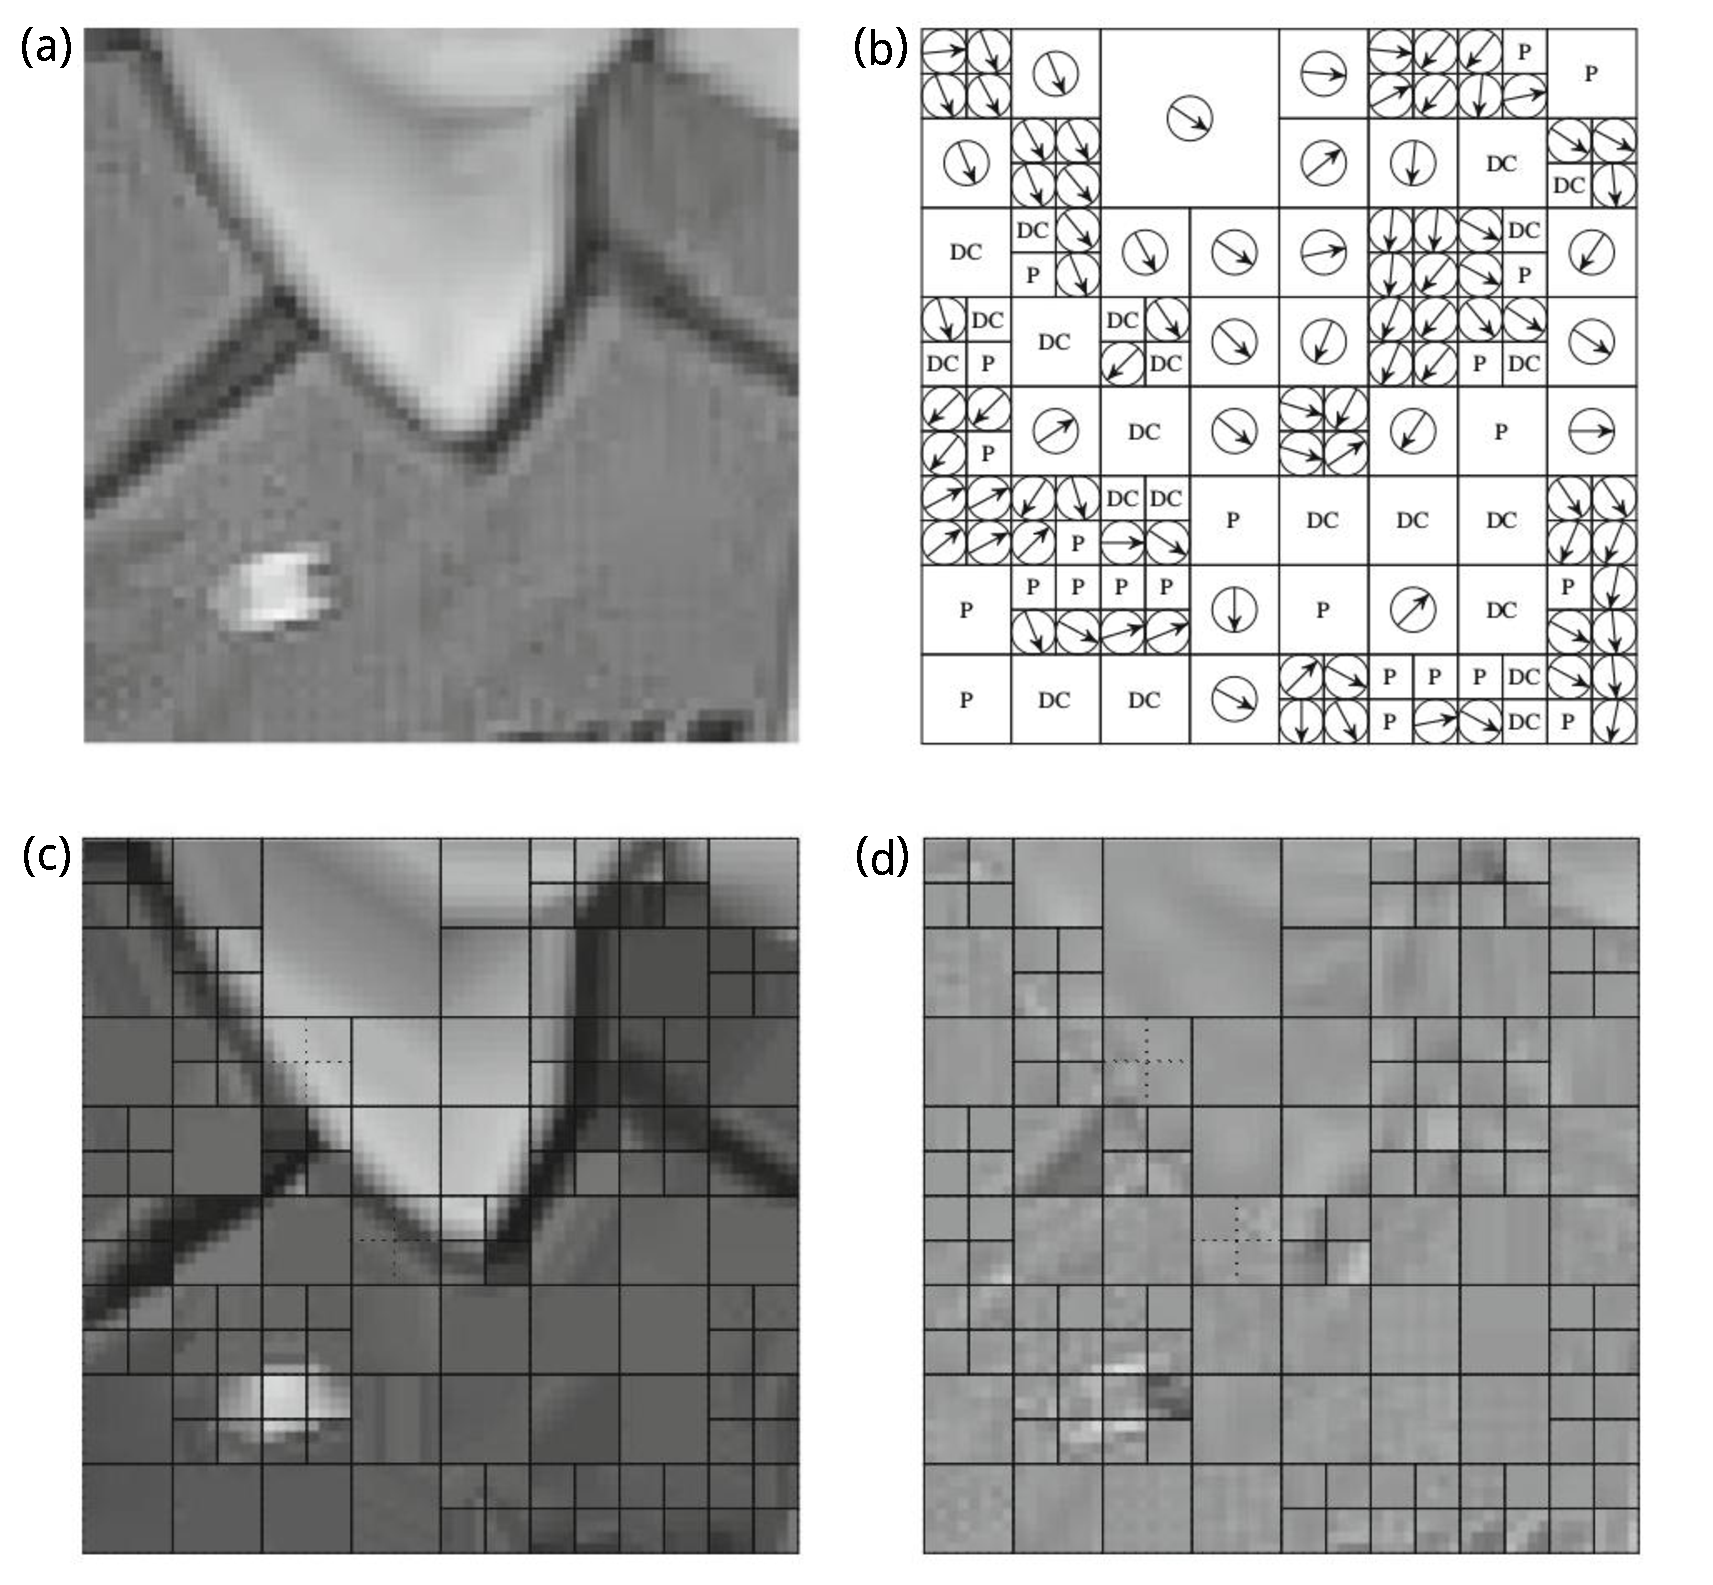
\includegraphics[scale=0.5]{Figures/Intra_coding_example}
  \caption[Esempio di predizione \emph{intra}]
          {CTB 64$\times$64 dove (a) è l'immagine originale, (b) i possibili
           modi di \emph{intra prediction} sulla base dei CU con predizione
           angolare (frecce), predizione planare ($P$) e predizione DC ($DC$).
           (c) rappresenta il segnale di predizione e (d) il residuo con il
           corrispondente CB (linee continue) e TB (linee tratteggiate).}
\end{figure}
%-------------------------------------------------------------------------------
%       SECTION 3
%-------------------------------------------------------------------------------

\section{Inter Prediction}\label{ref-inter}
L'\emph{inter prediction} sfrutta la correlazione temporale dei frame per 
ottenere una \emph{motion compensated prediction} (MCP), ovvero un PB predetto 
a partire da PB ``predittori'' che appartengono a frame precedentemente 
decodificati, supponendo che siano traslati nel PB predetto:
% Con questa frase volevo far capire che i PB "predittori" si sono spostati 
%fisicamente nel posto dove sta il PB predetto, non solo dire che si sono 
%traslati 

\begin{figure}[H]
  \centering
  \captionsetup{justification=raggedright}
  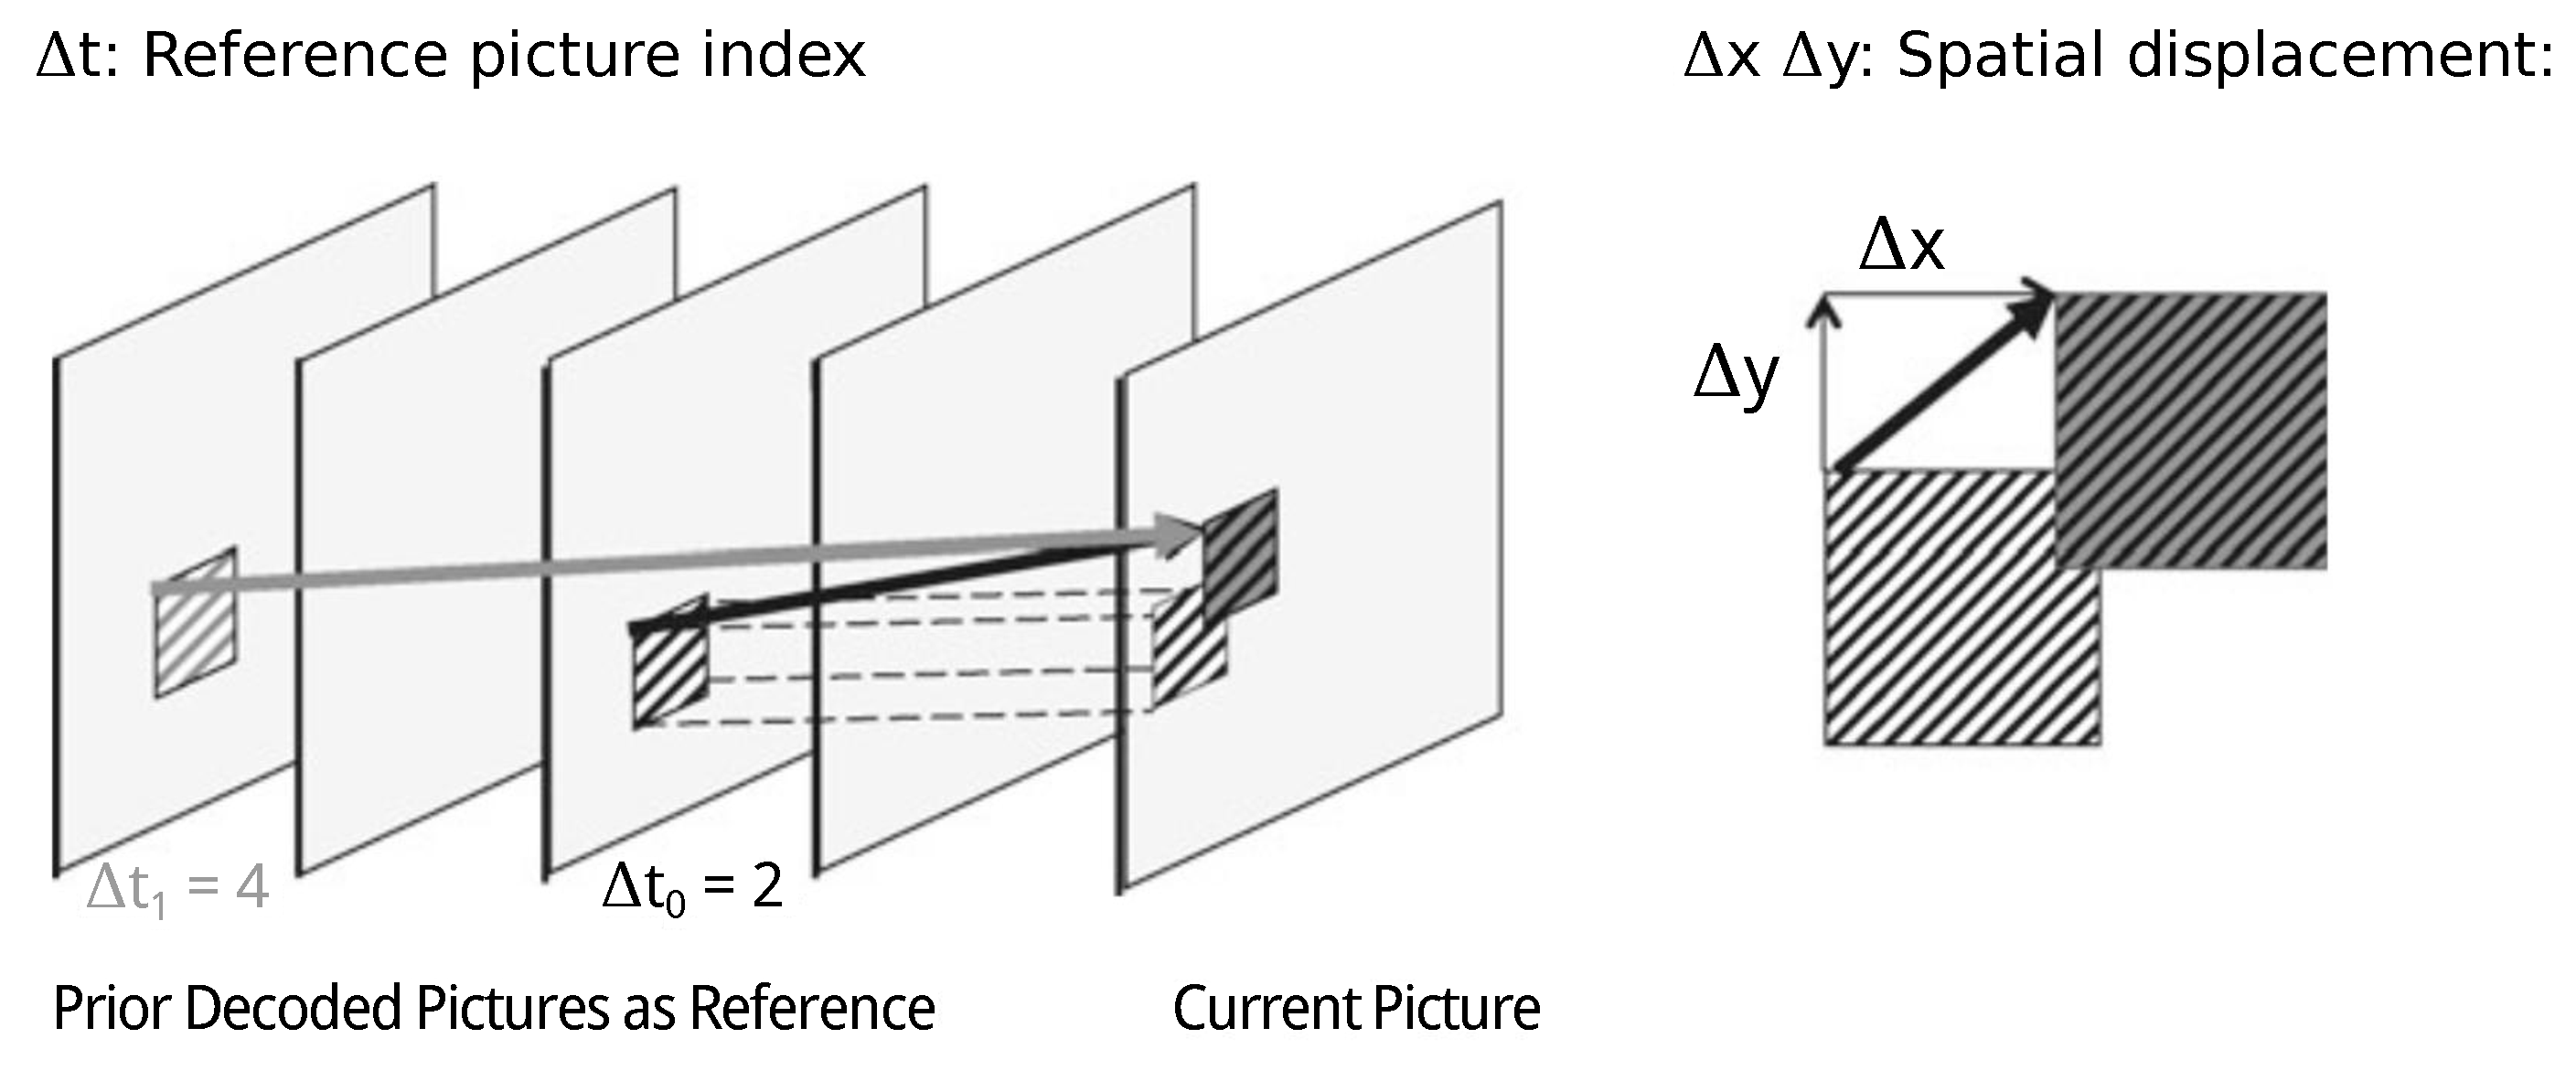
\includegraphics[scale=0.3]{Figures/Inter_pred}
  \caption{Concetti e parametri della \emph{inter prediction}}
\end{figure}

Per ogni PB l'encoder ricava un vettore ${(\Delta x,\Delta y,\Delta t)}$ 
chiamato \emph{motion data}, dove ${(\Delta x,\Delta y)}$ è il 
\emph{motion vector} e indica la traslazione compiuta dal PB in questione, 
mentre ${(\Delta t)}$ è l'indice temporale dell'immagine a cui appartiene il PB 
predittore.
È anche possibile effettuare una ``bipredizione'': in questo caso si usano 
due \emph{motion data} ottenendo due MCP di cui viene ricavata la media (che 
può anche essere pesata) per ottenere il risultato, come illustra la figura 
precedente.
\\ \\
Viene inoltre sfruttata la correlazione spaziale (ma sempre legata al tempo) 
dei \emph{motion vector}, basata sulla supposizione che i \emph{motion vector} 
relativi a PB spazialmente vicini non differiscano eccessivamente, eccezion 
fatta per eventuali punti di discontinuità come i cambi di oggetto. È inoltre 
ipotizzata una discreta continuità nel tempo per quanto riguarda i movimenti 
dell'intero \emph{frame}, escludendo variazioni brusche come i cambi di scena.
\\ \\
Tutto questo viene tradotto nel concetto di \emph{motion vector predictor} 
(MVP); invece di trasmettere un \emph{motion vector} per ogni PB l'encoder 
trasmette l'errore o la \emph{motion vector difference} (MVD), tra quello 
predetto a partire da blocchi spazialmente o temporalmente contigui e quello 
normalmente calcolato con $MVD=MV-MVP$.
Il decoder riceve la MVD e la sintassi necessaria a determinare il MVP (ovvero 
il tipo di predizione da utilizzare) e può dunque ricavare $MV$ come $MVD+MVP$.
 
Sebbene anche gli algoritmi che hanno preceduto H.265 (H.264 AVC) %H.264 
%Advanced 
%Video Coding è una cosa sola, qui ho sbagliato io nei riassunti
possiedano questo 
tipo di predizione, essi si limitano a calcolare $MVP$ come una media dei $MV$ 
vicini spazialmente: questa strategia non è più applicabile in HEVC a causa 
dell'elevata flessibilità delle strutture di predizione.
Il \emph{worst case scenario} presenta 16 $MV$ per lato da tenere in 
considerazione (come mostrato nell'immagine successiva), che porterebbe a 
complessità di codifica troppo elevate.

\begin{figure}[H]
  \captionsetup{justification=raggedright}
  \centering
  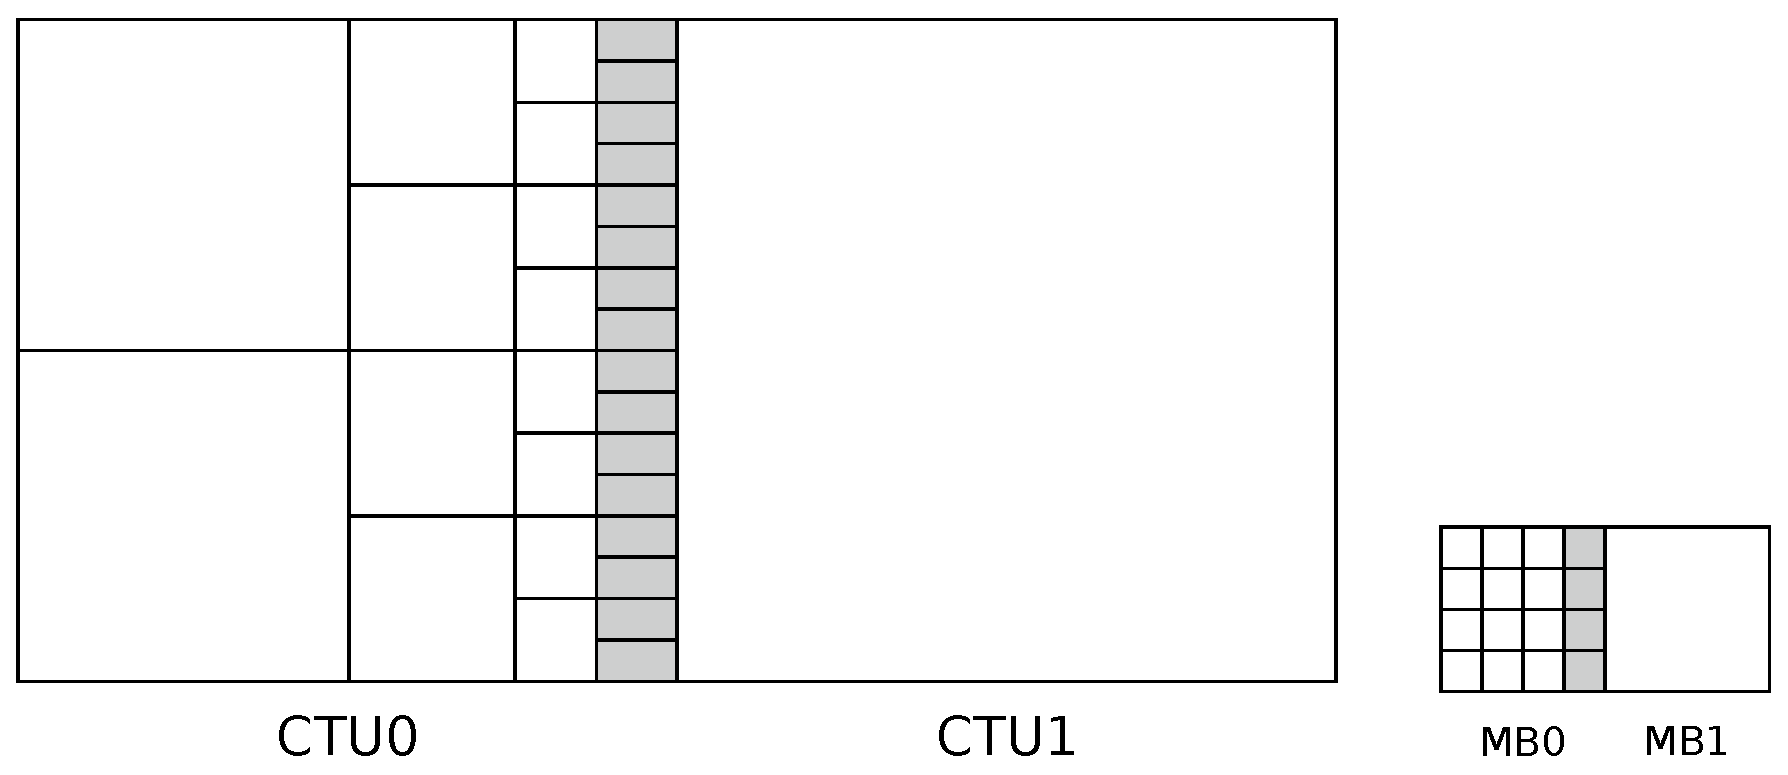
\includegraphics[scale=0.45]{Figures/Inter_pred_2}
    \caption[Numero massimo di \emph{motion vector} in H.265 e H.264]
    {Numero massimo di \emph{motion vector} in H.265 (a sinistra) e H.264 \\
      (a destra). CTU0 possiede 16 PB Luma 8x4 contigui a CTU1 che è composto da
      un solo PB Luma 64x64. MB0 (\emph{Macro Block)} contiene quattro 
      partizioni di predizione 4x4 affiancate a MB1 che consta di una 
      partizione 16x16. }
\end{figure}

H.265 mette a disposizione un algoritmo per la costruzione di vettori 
\emph{candidate MVP} chiamato \emph{advanced motion vector prediction} (AMVP), 
ottenuto in seguito ad esperimenti esaustivi volti a trovare predizioni che 
minimizzassero la complessità di codifica pur mantenendo buoni livelli di 
predizione (i.e., bassa entropia del segnale di errore MVD).
\\ \\
Una parte della sintassi di HEVC serve a comunicare al decoder quale MVP 
utilizzare tra quelli candidati, che sono due e scelti nei modi seguenti:
\begin{itemize}
\item Due \emph{spatial candidate} che derivano da cinque blocchi spazialmente 
vicini;
\item Viene tenuto come riserva un \emph{temporal candidate} derivato da due 
blocchi co-locati e temporalmente vicini:
\begin{itemize}
\item Nel caso che i due \emph{spatial candidate} siano uguali o uno di 
loro
 non sia disponibile, i due vettori candidati saranno uno spaziale e uno 
temporale;

\item Se entrambi i candidati spaziali non fossero disponibili, verrà 
considerato il vettore candidato temporale di riserva ed uno 
\emph{zero motion vector};

\item Nell'eventualità che sia i candidati spaziali sia i candidati temporali 
non siano disponibili, entrambi i candidati saranno \emph{zero motion vector}.
\end{itemize}
\end{itemize}

Gli \emph{spatial candidate} sono ottenuti prendendo in considerazione cinque 
blocchi spazialmente vicini suddivisi in due gruppi: il primo contenente i 
due blocchi in basso a sinistra rispetto a quello che si vuole predire, il 
secondo con i tre blocchi in alto.
% I nomi A e B facevano riferimento ad un'immagine che non è stata usata
Generalmente, se i vettori dei blocchi considerati sono riconducibili allo 
stesso \emph{reference id} (l'indice dell'immagine a cui fanno 
riferimento) di quello del blocco che si vuole predire, tali vettori saranno 
MVP.
Viceversa, MVP sarà il vettore scalato secondo una formula che dipende dalla 
differenza temporale dei \emph{reference id}.
Non sono invece presi in considerazione blocchi a destra o in basso dal 
momento che tali PB non sono ancora stati decodificati e non sono disponibili 
al decoder per la predizione.
\\ \\
Per quanto concerne il \emph{temporal candidate} si lavora su una immagine 
co-locata e temporalmente vicina della quale, in fase di decodifica, si 
possiedono tutte le informazioni (ovvero un frame già decodificato); diversi 
esperimenti hanno dimostrato che i blocchi da prendere in considerazione sono 
due: quello al centro e quello in basso a destra rispettivamente alla posizione 
del blocco che si vuole predire.
Specificamente il vettore viene predetto utilizzando sempre il blocco in basso 
a destra, salvo la mancanza di disponibilità d quest'ultimo; ciò significa che 
esso risiede fuori dai bordi dell'immagine o viola vincoli imposti per motivi 
di memoria.
\\ \\
Infine HEVC risolve un problema legato alla struttura di suddivisione delle 
immagini \emph{quadtree}: quest'ultime permettono una grande flessibilità 
delle dimensioni dei blocchi con un basso costo di \emph{overhead} in termini 
di \emph{bit rate}. Per l'\emph{inter prediction} la struttura a \emph{quadtree}
 permette di suddividere minuziosamente quelle parti di immagine che presentano 
bruschi movimenti rispetto alle parti più statiche che non richiedono una 
grande informazione di movimento. Questo tipo di raggruppamento, tuttavia, 
origina facilmente bordi ineffettivi (\emph{over segmentation}); HEVC dispone 
di un  algoritmo di \emph{block merging} che consente di raggruppare PB con 
uguali parametri di predizione in modo da trasmetterne una sola copia.

\begin{figure}[H]
  \centering
  \captionsetup{justification=raggedright}
  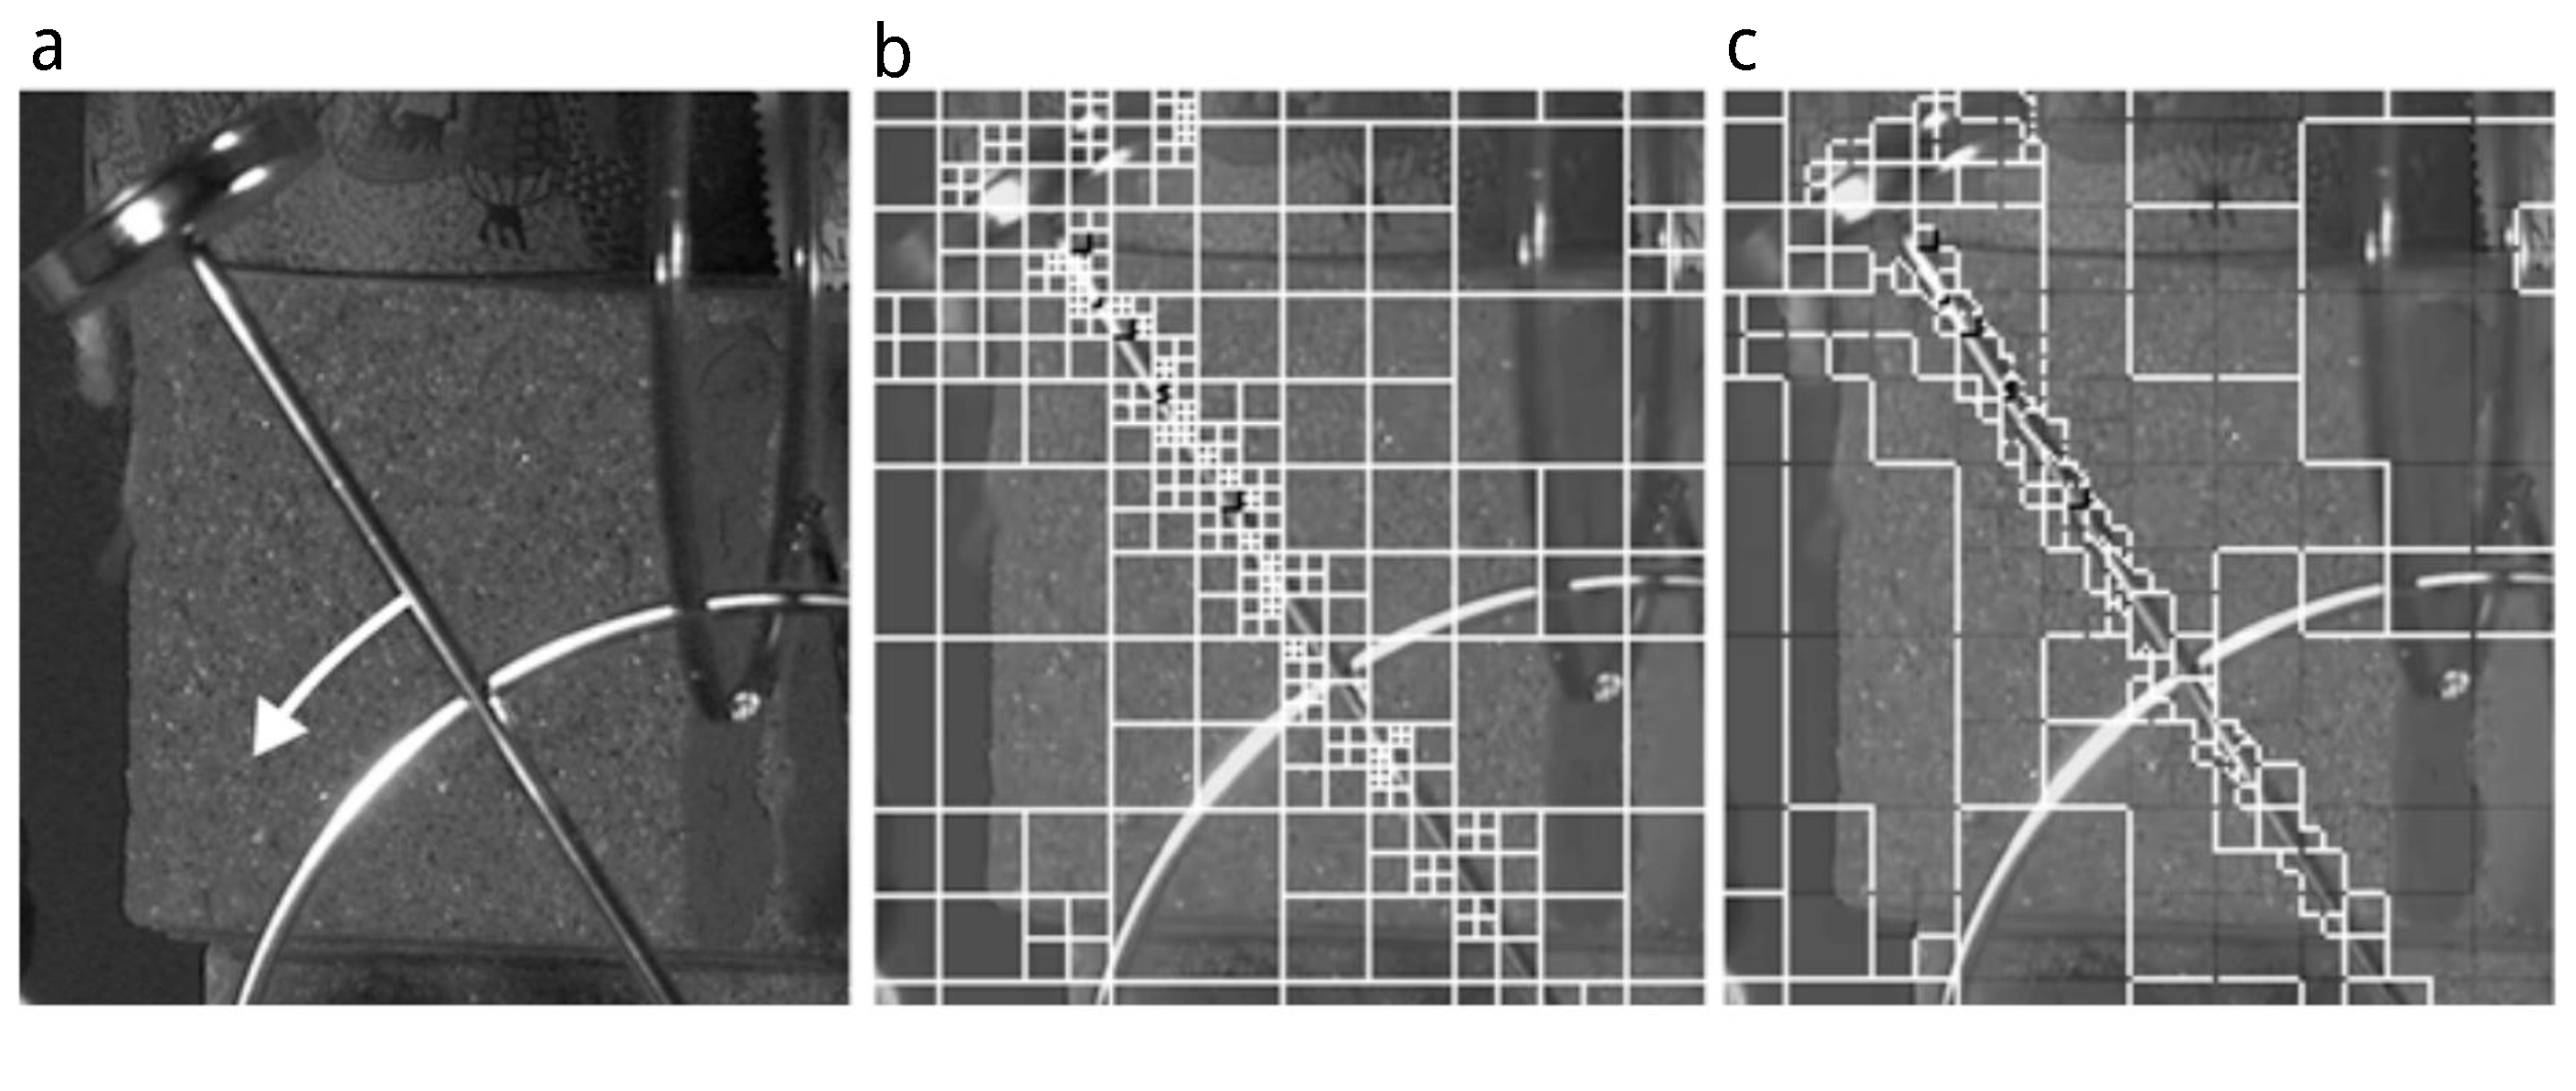
\includegraphics[scale=0.30]{Figures/Block_merging}
  \caption[Esempio di \emph{block merging}]
          {Esempio di \emph{block merging} dove a) è l'immagine originale, b)
           l'immagine scomposta in PB secondo la struttura a \emph{quadtree}
           mentre c) mostra il risultato del \emph{block merging}}
\end{figure}
%-------------------------------------------------------------------------------
%       SECTION 4
%-------------------------------------------------------------------------------
\newpage
\section{Transform and Quantization}
Nel \emph{block-based video coding} i segnali di errore residui che derivano 
dalle predizioni intra o inter vengono trasformati e quantizzati prima di 
essere trasmessi.
Più nel dettaglio, un'immagine è suddivisa in blocchi quadrati di dimensione 
$N{\times}N$, dove $N=2^M$ con $M \in \mathbb{N}$. Per ogni blocco esisterà un 
blocco 
residuo $U$ che verrà trasformato e quantizzato. \\
%L'immagine mostra il percorso dei dati durante la fase di encoding (a) e 
%di decoding (b):
\begin{figure}[H]
  \centering
  \captionsetup{justification=raggedright}
  \begin{tabular}{cc}
    \subfloat[]{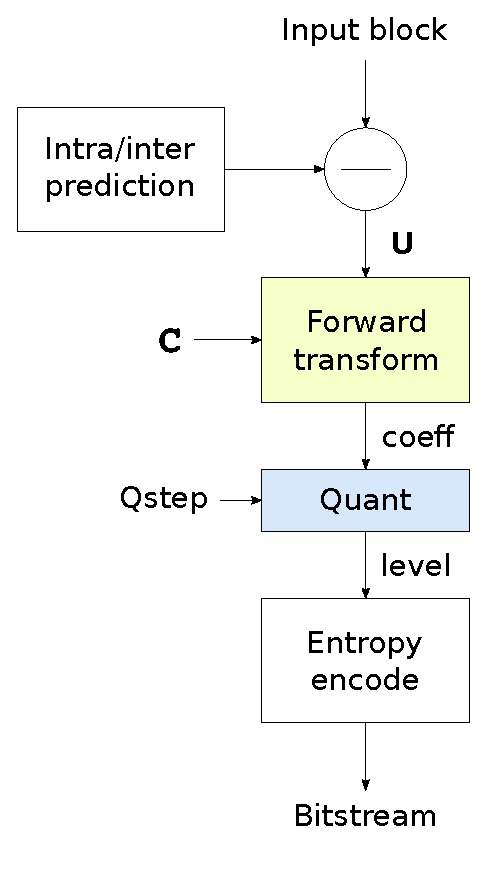
\includegraphics[scale=.66]{Figures/Transf_and_quant_a}}
    &\qquad
    \subfloat[]{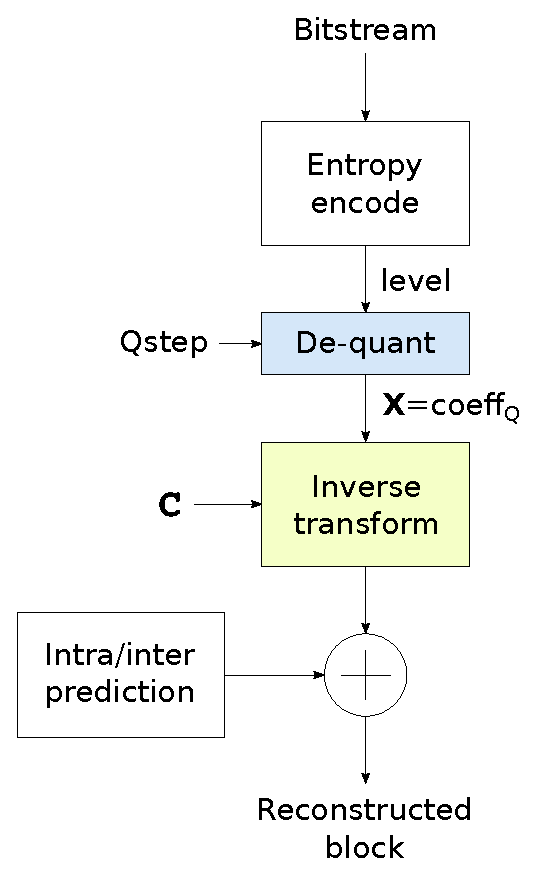
\includegraphics[scale=.66]{Figures/Transf_and_quant_b}}
  \end{tabular}
  \caption[\emph{Data flow} di encoding e decoding.]
          {\emph{Data flow} di encoding e decoding, dove a) mostra il percorso
           in fase di encoding e b) quello in fase di decoding.}
\end{figure}

%-----------------------------------
%       SUBSECTION 1
%-----------------------------------

\subsection{Transform}
Tipicamente le trasformate sono delle matrici costruite in modo tale che, in 
assenza di quantizzazione, sommando trasformata e trasformata inversa si 
ottenga un risultato praticamente lossless.
HEVC utilizza due tipologie di trasformate, ovvero quelle derivate dalla DCT e
quelle derivate dalla DST; fornisce inoltre delle matrici precostruite per 
eseguire l'antitrasformata DCT e DST per tutte le possibili dimensioni dei 
blocchi: $4{\times}4$, $8{\times}8$, $16{\times}16$ e $32{\times}32$.
Queste matrici contengono approssimazioni ad interi con precisione finita dei 
coefficienti di trasformazione DCT-II; questo sistema riduce di molto la 
complessità di \textit{encoder} e \textit{decoder}, e risolve un problema che 
era presente in H.261, ovvero la deriva dovuta a lievi disallineamenti nella 
rappresentazione \textit{fixed point} dei coefficienti tra la matrice di 
trasformazione, costruita arbitrariamente dall'implementatore 
dell'\textit{encoder}, e quella di antitrasformazione fornita dallo standard. \\
Errori di questo tipo si ripercuotono amplificati in ogni immagine successiva, 
costringendo a dover trovare un modo di ovviare al problema (il sopracitato 
H.261 costringeva un aggiornamento periodico del segnale che consisteva in una 
immagine codificata interamente intra).

%-----------------------------------
%       SUBSECTION 2
%-----------------------------------

\subsection{Quantization}
Con ``quantizzazione'' si intende la divisione dei valori trasformati 
utilizzando un passo di quantizzazione $Q_s$ (\emph{quantization step}) definito
 attraverso il parametro di quantizzazione $Q_p$ come segue:
\begin{align*}
Q_s = \left(2^{\frac{1}{6}}\right)^{(Q_p-4)}
\end{align*}
Dalla formula si può notare come una variazione di $1$ per $Q_p$ si traduca in 
una moltiplicazione di $Q_s$ per un fattore $2^{\frac{1}{6}}\approx 1.12$, ovvero 
nell'incremento di $Q_s$ del $12\%$. Una variazione di $6$ si traduce in un 
raddoppiamento di $Q_s$ \\
Si può anche eseguire una quantizzazione \emph{frequency dependent} specificando
 una matrice $\omega$ con un valore di quantizzazione per ogni frequenza, con 
 un 
risultato che risulta il seguente:
\begin{align*}
q[x][y] = \frac{tc[x][y]}{\omega[x][y]\cdot Q_s}+offset
\end{align*}
dove $tc$ sono i coefficienti trasformati. \\
Si ottiene una compressione in quanto i valori, una volta quantizzati, verranno 
arrotondati all'intero più vicino. Il fine è quello di portare a 0 il maggior 
numero possibile di coefficienti in modo che la codifica successiva (marcata 
come \emph{Entropy encode}) sia in grado di comprimere al meglio la sequenza in 
uscita; con $\omega$ si può agire sul denominatore, dividendo un intero per un 
numero più grande il risultato sarà più 
vicino a zero. Tipicamente le matrici di quantizzazione possiedono valori più 
piccoli alle basse frequenze e viceversa alle alte, perché il contenuto utile 
per il sistema visivo umano è concentrato alle basse frequenze.
%dividendo le basse frequenze per valori piu grandi le rendo 0

%-------------------------------------------------------------------------------
%       SECTION 5
%-------------------------------------------------------------------------------

\section{In-Loop Filters}
Lo standard ibrido di codifica HEVC scompone i frame attraverso una struttura a 
blocchi per effettuare la compressione; questa suddivisione porta spesso alla 
comparsa di artefatti che danno alle sequenze video un aspetto quadrettato, 
peggiorandone la qualità visiva. Un esempio tipico di causa della discontinuità 
tra i blocchi è la predizione inter di due blocchi contigui che nel frame
 di riferimento erano distanti, oppure anche la codifica di due blocchi contigui
 con modalità predittive differenti (due intra diversi, una inter e una intra, 
etc.). Per porre rimedio a questi artefatti lo standard HEVC specifica due 
filtraggi: il \emph{deblocking filter} e il \emph{sample adaptive offset} (SAO).
\\ \\
Questi filtraggi sono chiamati \emph{in-loop filters} perché vengono eseguiti 
all'interno dei cicli di \textit{encoding}/\textit{decoding}, e i risultati 
vengono utilizzati nei cicli successivi oltre che durante la visualizzazione 
delle sequenze decodificate; in questo modo si trae vantaggio dalla procedura 
di filtraggio anche durante il \textit{decoding} dei \textit{frame} successivi, 
perché le predizioni inter vengono effettuate a valle di \textit{frame 
reference} di maggiore qualità.
\\ \\
Il \emph{deblocking filter} si occupa di smussare i confini tra due blocchi in 
cui è presente una discontinuità, cercando di lavorare solo su quelle 
introdotte durante la compressione e non quelle originariamente presenti nella 
sequenza. \\
Il SAO, invece, si occupa di ridurre gli artefatti dovuti a trasformazioni e 
quantizzazioni grossolane (chiamati \emph{ringing artifacts}), ed opera 
sull'output del \emph{deblocking filter} in cascata. \\
Visto che i due filtraggi operano su due artefatti diversi, i loro benefici 
sono additivi se eseguiti insieme.

%-----------------------------------
%       SUBSECTION 1
%-----------------------------------

\subsection{Deblocking Filter}
Il \emph{deblocking filter} si applica solo ai confini tra blocchi di tipo CU, 
PU o TU e non al loro interno; durante la codifica  l'\textit{encoder} 
considera gruppi di quattro vettori di campioni perpendicolari ai confini dei 
blocchi. 
Specificamente l'\textit{encoder} esegue alcuni controlli sul primo e sul 
quarto vettore per decidere:
\begin{itemize}
\item Se eseguire il filtraggio o meno;
\item In caso positivo quale filtraggio applicare tra \textbf{normal} e 
\textbf{strong}.
\end{itemize}
Questi semplici controlli misurano un indice di distorsione dei vettori di 
campioni rispetto ad una delle funzioni continue più semplici, ovvero una rampa 
che attraversa il confine. Se questo indice supera 
una certa soglia, che dipende dal passo di quantizzazione $Q_p$ secondo una 
\emph{look-up table}, si esegue il filtraggio.

\begin{figure}[H]
  \captionsetup{justification=raggedright}
  \centering
  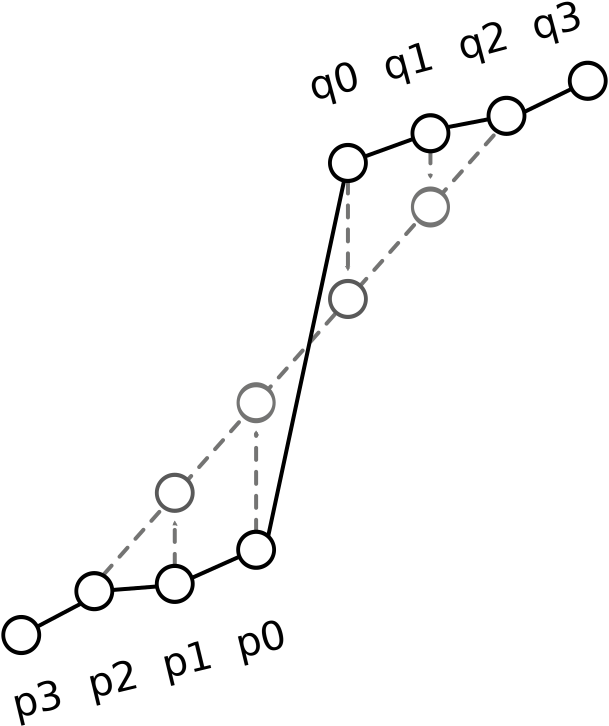
\includegraphics[scale=0.3]{Figures/Deblocking_filter}
  %era veramente troppo grande
    \caption[Filtraggio \emph{deblocking} di tipo \textbf{normal}]
    {Filtraggio \emph{deblocking} di tipo \textbf{normal}: la linea nera mostra
      il confine originale del blocco, la linea grigia tratteggiata quello 
      nuovo}
\end{figure}

L'immagine mostra il risultato di un filtraggio \textbf{normal} eseguito su un 
vettore di 8 campioni, con questi ultimi appartenenti a due blocchi confinanti 
chiamati $P$ e $Q$.
In generale, un filtraggio \textbf{normal} può arrivare a modificare fino a due
campioni per lato avvicinandoli alla rampa, come accade nell'immagine.
Il filtraggio \textbf{strong} viene utilizzato nelle aree che racchiudono 
contenuti a bassa frequenza, ovverosia quelle in cui il sistema visivo umano è 
più sensibile alle discontinuità, e consiste in un filtraggio lineare lowpass 
che comprende tre campioni per lato.
\\ \\
Il filtraggio \emph{deblocking} descritto interessa solamente il canale luma, 
dal momento che per i canali chroma si opera un filtraggio analogo ma più 
grossolano, in cui vengono eseguiti molti meno controlli e vengono considerati 
meno campioni: ciò permette di ridurre la complessità dell'encoder a fronte di 
una bassa perdita di qualità, sempre considerando il fatto che i canali chroma 
sono meno importanti per il sistema visivo umano.

\begin{figure}[H]
  \centering
  \captionsetup{justification=raggedright}
  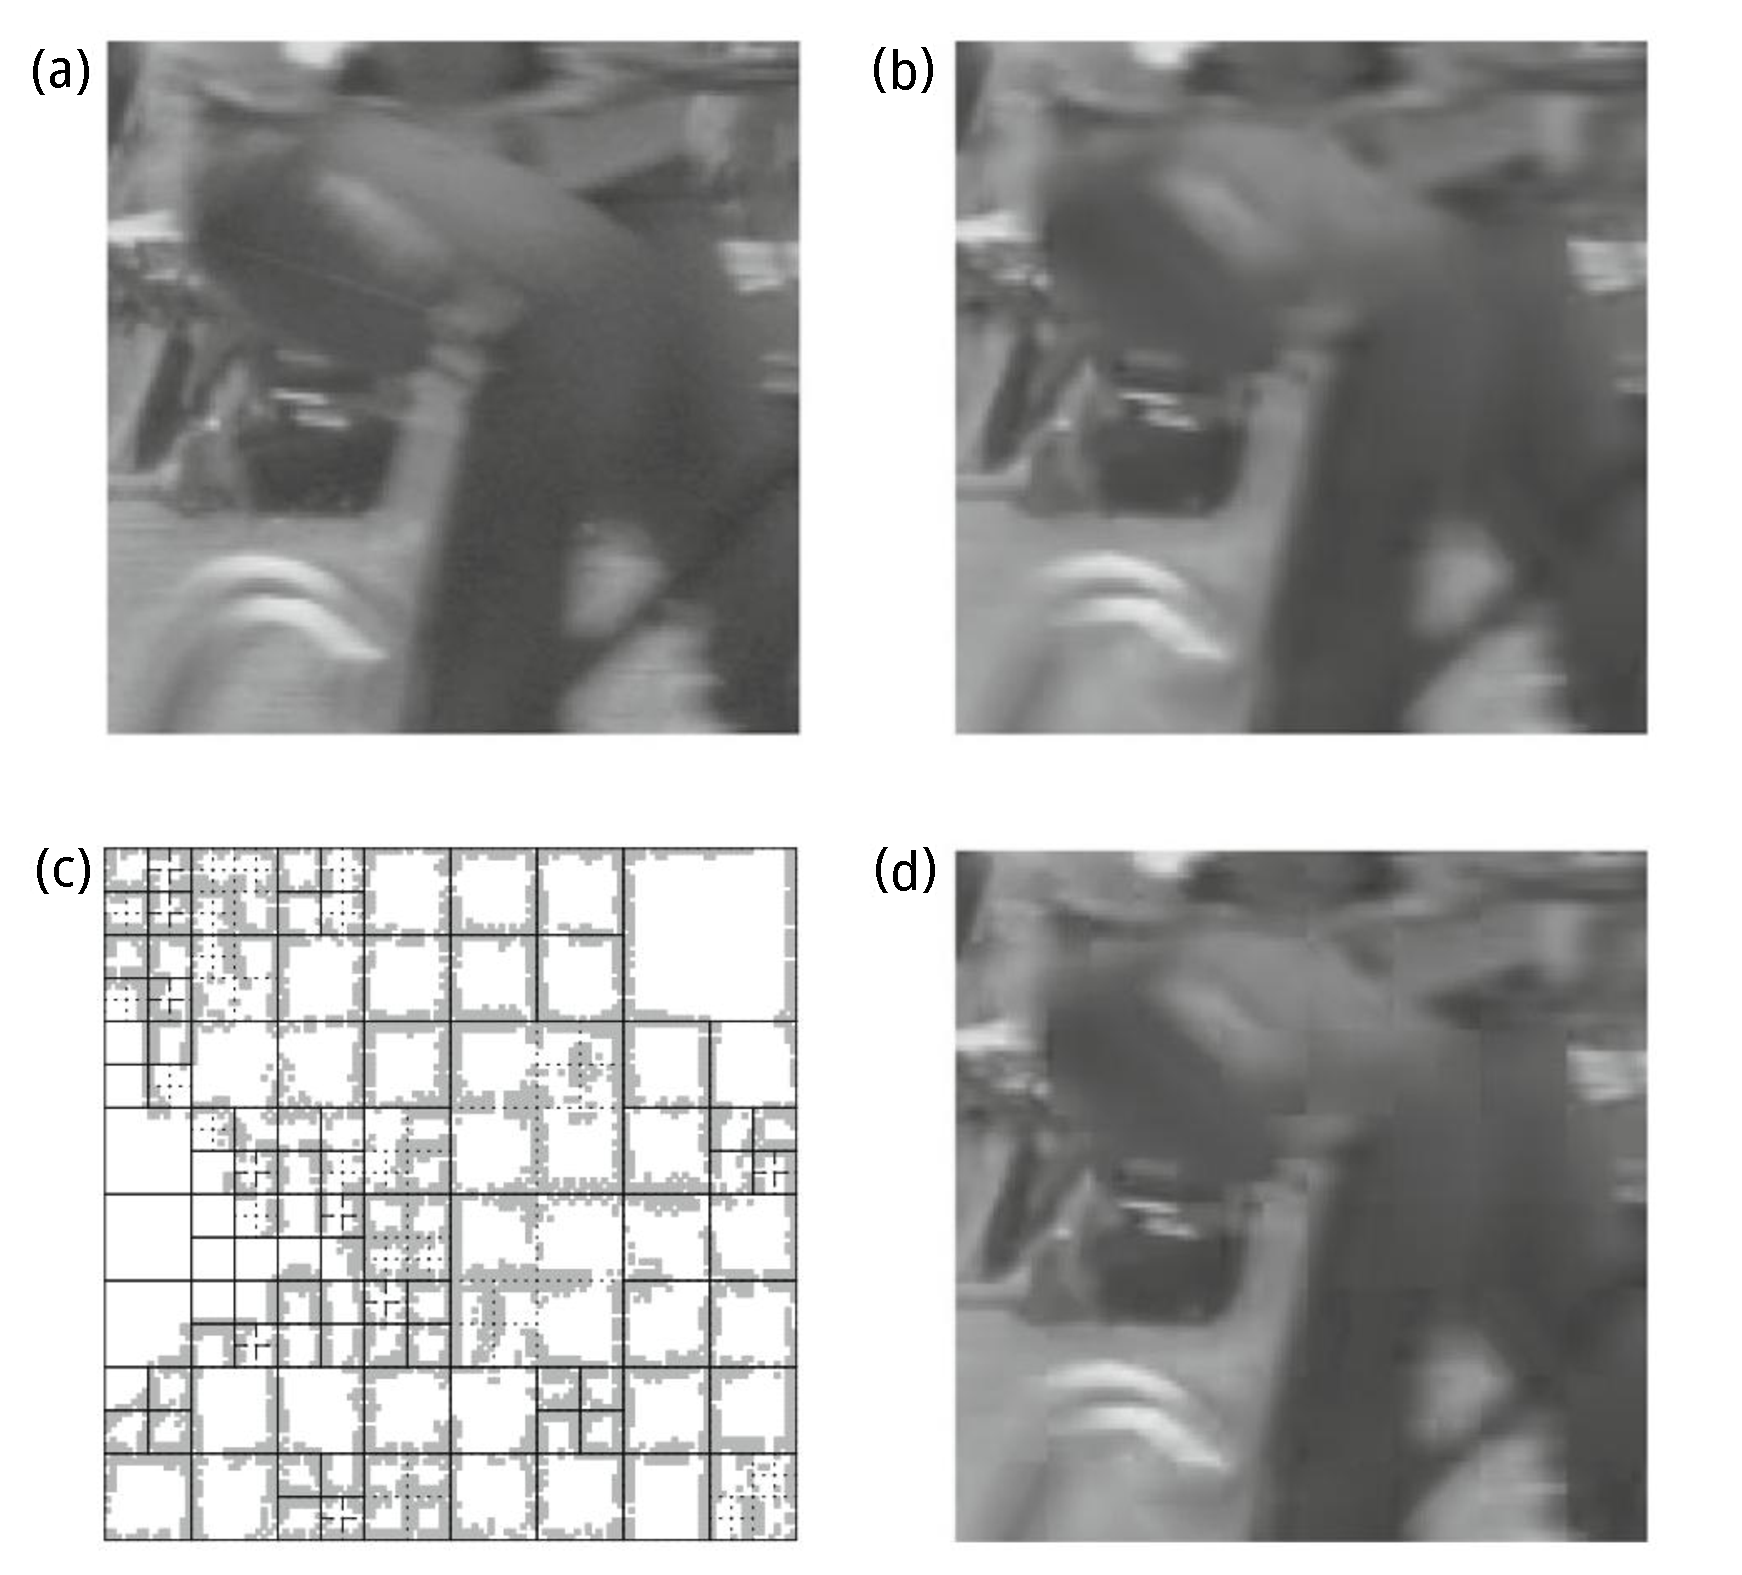
\includegraphics[scale=.42]{Figures/deblocking_filter_example}
  %una volta stampata, questa era visivamente più grande dell'img originale
  \caption[Esempio di \emph{deblocking filtering}]
          {Esempio di \emph{deblocking filtering} per un CTB, dove le linee
           continue rappresentano i CB, le linee tratteggiate i PB e le linee
           puntinate i TB. a) è l'immagine originale, b) l'immagine ricostruita
           con il \emph{deblocking}, c) la struttura di CB, PB e TB e d) 
           presenta una ricostruzione senza l'utilizzo del \emph{deblocking}.}
\end{figure}

%-----------------------------------
%       SUBSECTION 2
%-----------------------------------

\subsection{Sample Adaptive Offset - SAO}
Il SAO è un filtraggio che mira ad eliminare i \emph{ringing artifacts} 
scaturiti dalla trasformazione e quantizzazione del segnale residuo, e 
comprende due tecniche di filtraggio: \emph{Edge Offset} (\textbf{EO}) e 
\emph{Band Offset} (\textbf{BO}).\\
La scelta tra questi due tipi di filtraggio avviene a livello di CTU, ricordando
che  algoritmi di \emph{merging} consentono di raggruppare più CTU con parametri
SAO uguali in modo tale da trasmetterne una sola copia, così da ridurre la 
ridondanza di informazioni collaterali.
\\ \\
L'\emph{edge offset} si occupa di compensare il fenomeno di Gibbs (\emph{Gibbs
phenomenon}) mostrato nell'immagine.

\begin{figure}[H]
  \centering
  \captionsetup{justification=raggedright}
  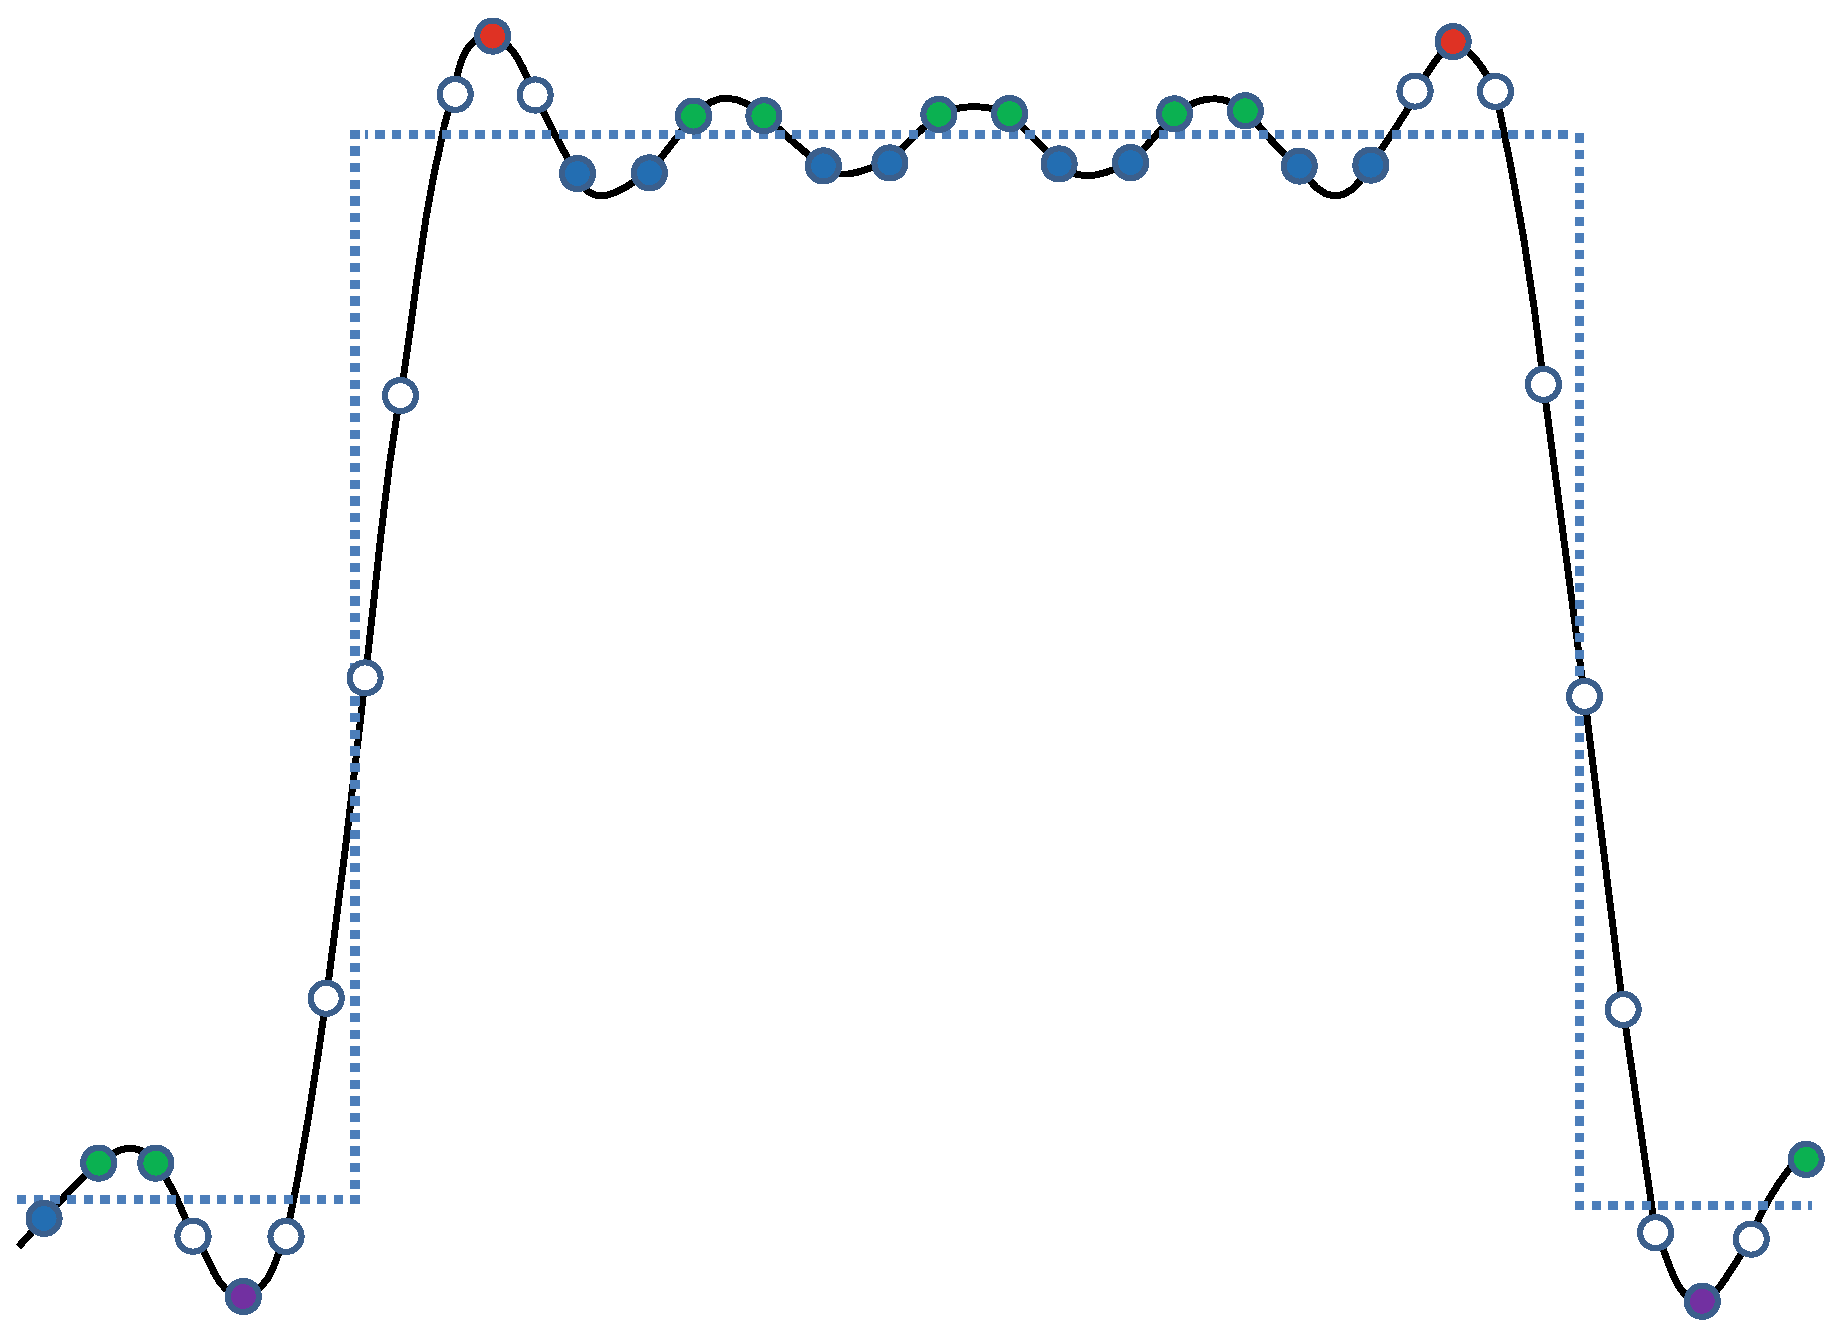
\includegraphics[scale=0.3]{Figures/SAO_Gibbs}
  \caption[Fenomeno di Gibbs]
  	  {Fenomeno di Gibbs, dove la linea tratteggiata rappresenta i
	   campioni originali mentre la linea continua mostra i campioni
	   ricostruiti.}
\end{figure}

Il taglio delle frequenze più alte comporta una distorsione che presenta valli e
picchi locali pronunciati; il filtraggio consiste inizialmente nella 
classificazione di ogni campione come valle locale, picco locale, angolo concavo
e angolo convesso (\emph{local peak/valley}, \emph{convex/concave corner}).
La classificazione viene fatta confrontando il valore del campione selezionato 
con quello dei due campioni vicini (detti \emph{neighbour}) che possono essere 
scelti lungo quattro direzioni: orizzontale, verticale, $45^{\circ}$ e 
$135^{\circ}$. In seguito, a seconda della classificazione, viene applicato un
\emph{offset} positivo o negativo al campione: per ogni blocco di filtraggio EO
l'encoder sceglie e comunica il modulo di quattro valori di offset (uno per ogni
classe), questo significa che all'interno di un unico blocco EO tutti i campioni
appartenenti alla stessa classe condividono lo stesso \emph{offset}.
\\ \\
Il \emph{band offset} è pensato per ridurre l'errore dovuto alla cattiva 
quantizzazione del residuo delle predizioni o a sfasamenti dei vettori di moto 
predetti rispetto a quelli reali. Questo tipo di errore risulta relativamente 
costante al variare dei campioni e può essere corretto, almeno in media, con un 
\emph{offset} costante, come mostrato in figura.

\begin{figure}[H]
  \centering
  \captionsetup{justification=raggedright}
	  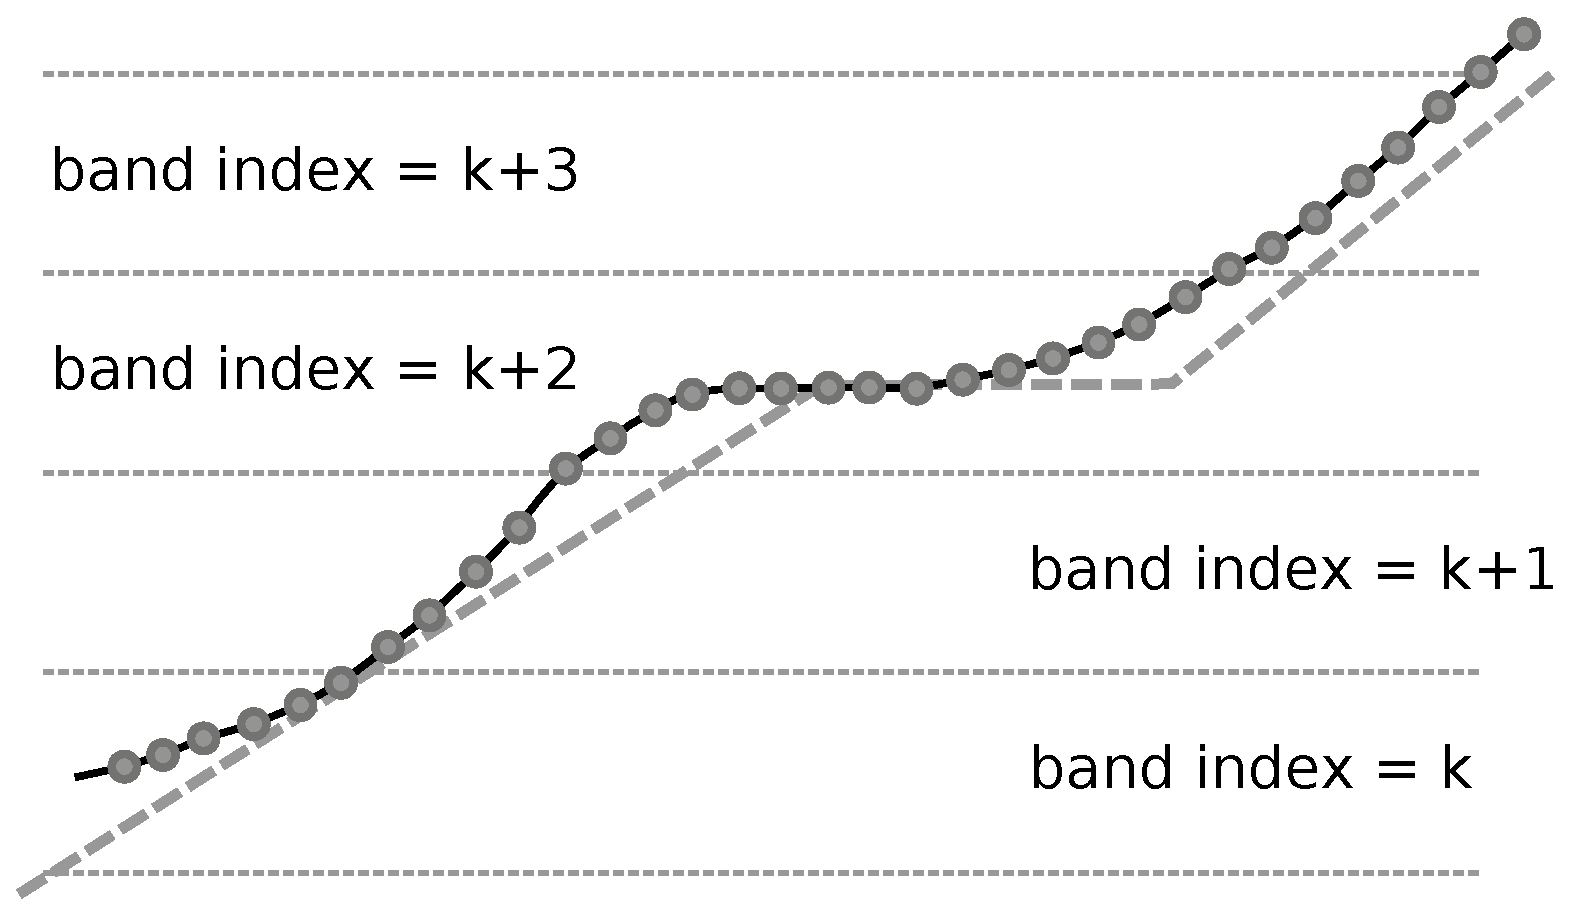
\includegraphics[scale=0.37]{Figures/Band_offset}
	  %abbiamo la fissa per le cose grosse, eh?
  \caption[Esempio di \emph{Band Offset}]
  	  {Esempio di \emph{Band Offset}, in cui la linea tratteggiata
	   rappresenta i campioni originali mentre la linea continua mostra
	   i campioni ricostruiti.}
\end{figure}

Eventualmente, HEVC permette ulteriori miglioramenti specificando quattro 
\emph{offset}. \\
Il range dei valori dei campioni viene suddiviso in 32 bande omogenee; se i 
campioni fossero ad 8 bit, con valori da 0 a 255, le bande avrebbero ampiezza 
pari a 8. A questo punto l'\textit{encoder} sceglie le quattro bande contigue 
che raccolgono la maggior percentuale di errore rispetto al segnale originale e 
determina quattro valori di offset, ovverosia uno per ogni banda. 
Successivamente viene applicato l'\emph{offset} corrispettivo a tutti i campioni
il cui valore rientra all'interno di una delle suddette quattro bande; per ogni 
blocco BO l'\textit{encoder} deve dunque comunicare l'indice della prima delle 
quattro bande e i valori di offset.

%-------------------------------------------------------------------------------
%       SECTION 6
%-------------------------------------------------------------------------------

\section{CABAC}
Il \emph{Context-Based Adaptive Binary Arithmetic Coding} (CABAC) è il blocco 
finale all'interno del ciclo di codifica che esegue una compressione 
\emph{lossless} sui dati binari che vengono posti subito dopo in uscita 
all'\textit{encoder}. La compressione si basa sulle proprietà statistiche dei 
dati relative al loro contesto di codifica (da qui il \emph{context-based}), 
cercando di rendere la dimensione in bit di una parola di codice proporzionale 
in modo logaritmico alla probabilità del dato che essa codifica (dal primo 
teorema di Shannon: la codifica ottima pesa $-log_2p$). \\
CABAC opera solamente sui \emph{syntax element} all'interno del \emph{binary 
stream}, ovvero quei dati che contengono principalmente i parametri che 
riguardano gli algoritmi di codifica; il suo compito è dunque quello di ridurre
l'\emph{overhead} della \emph{side information} dovuta alla flessibilità 
dell'\textit{encoder} video ibrido. \\

\begin{figure}[H]
  \centering
  \captionsetup{justification=raggedright}
  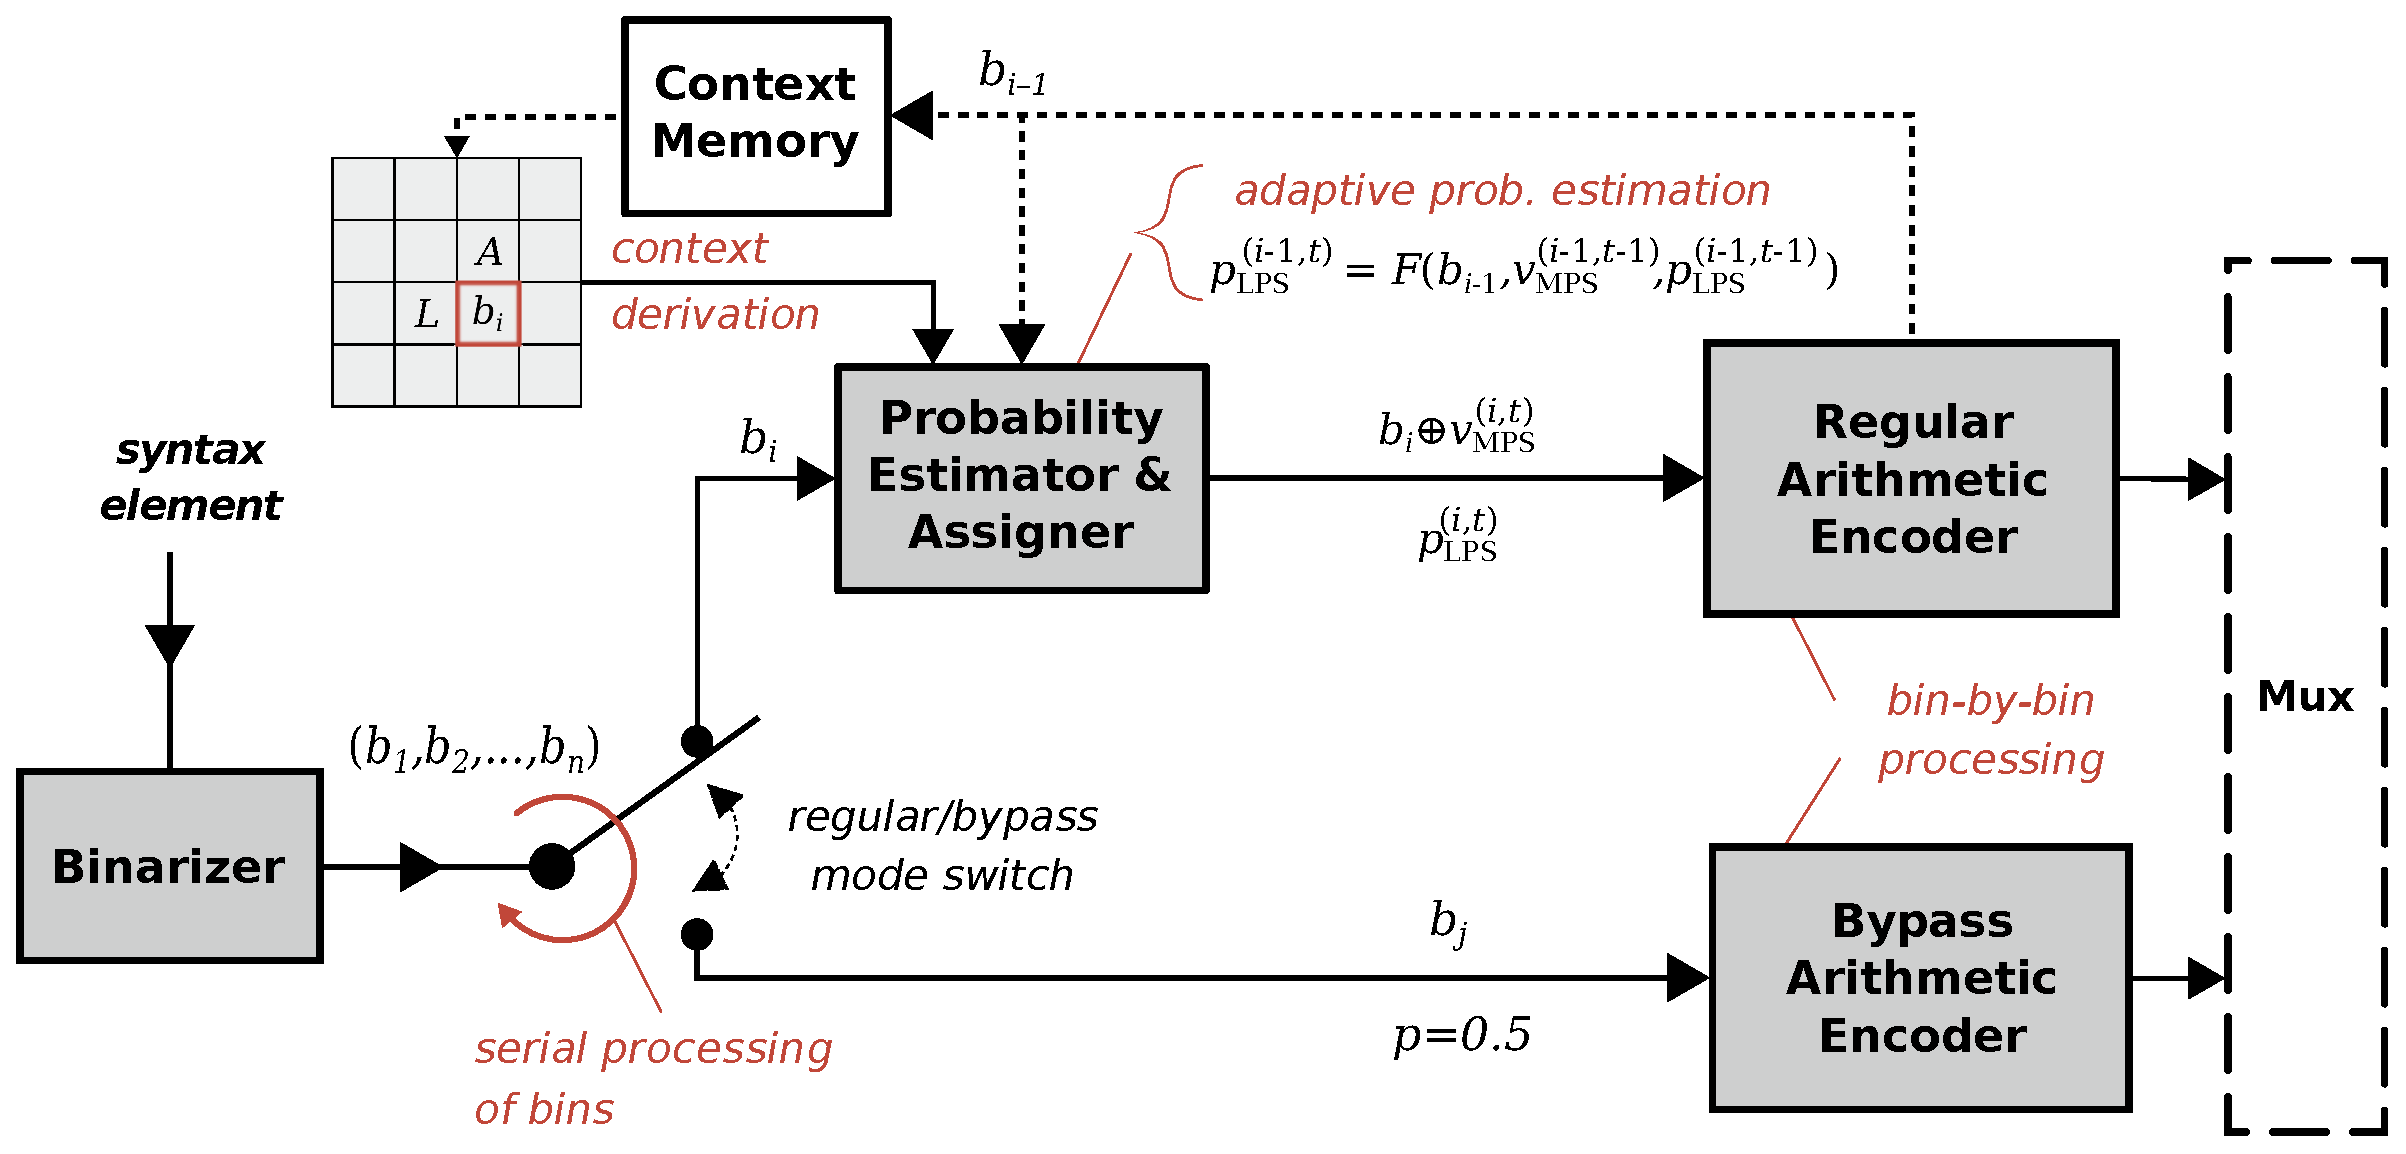
\includegraphics[scale=0.35]{Figures/Cabac_overview}
  \caption[Percorso di un \emph{syntax element} dentro CABAC]
	  {Percorso di un singolo \emph{syntax element} all'interno di CABAC,
	   con i possibili colli di bottiglia segnati in rosso.}
\end{figure}

Il primo passaggio consiste nella binarizzazione del \emph{syntax element} 
sostituendolo con una stringa di simboli binari; successivamente si verifica 
la parte \emph{context-based}, ovvero l'assegnazione di una probabilità ad ogni 
simbolo. Infine la stringa di simboli relativi al \emph{syntax element} viene 
codificata (i.e., associata alla parola di codice) tramite codifica aritmetica e
posta in uscita.
%-----------------------------------
%       SUBSECTION 1
%-----------------------------------

\subsection{Binarization}
Uno schema di binarizzazione è una mappa che associa ad ogni valore numerico 
un'unica sequenza di cifre binarie (chiamate ``bins'', \emph{binary symbols}) 
in maniera univocamente decifrabile. Lo schema di binarizzazione viene scelto a
seconda del tipo di \emph{syntax element}, con gli schemi principali che 
risultano essere i seguenti:
\begin{itemize}
\item \emph{Fixed Length}: un valore numerico viene rappresentato con la 
  classica numerazione a base binaria. Se si usassero tre bin si potrebbero 
  mappare fino a otto valori: $0 \rightarrow 000$, $1 \rightarrow 001$, 
  {\ldots}, $6 \rightarrow 110$, $7 \rightarrow 111$

\item \emph{Unary} (U): per rappresentare il numero $N$ si utilizzano 
  esattamente $N$ simboli $1$ seguiti da uno $0$, ad esempio $5 \rightarrow 
  111110$

\item \emph{Truncated Unary} (TrU): considerando $cMax$ il valore massimo che 
  si desidera binarizzare, verrà effettuata una binarizzazione \emph{Unary} 
  per tutti i numeri eccezion fatta per $cMax$ che non verrà terminato con $0$.

\item \emph{K-th Order Truncated Rice} (TRk): Sia N il numero che si vuole 
  binarizzare $\Rightarrow V = \left\lfloor\frac{N}{2^k}\right\rfloor$. In 
  questo modo sono stati rimossi i $k$ bit meno significativi di $N$; il 
  risultato si ottiene affiancando alla rappresentazione \textbf{TrU} di $V$ 
  quella \emph{Fixed Length} del valore dei $k$ bit meno significativi.

\end{itemize}
%-----------------------------------
%       SUBSECTION 2
%-----------------------------------

\subsection{Context Modeling}\label{ref-context-modeling}
Questa è la fase in cui avvengono tutte le decisioni \emph{context-based}, tra
cui la prima è la scelta della modalità di codifica che può essere 
\emph{regular} o \emph{bypass}. Nel secondo caso si suppone una densità di 
probabilità
uniforme e si associa $0.5$ di default ad ogni bit. La codifica \emph{regular}
può invece dare una probabilità basata sul tipo di \emph{syntax element} e sulla
posizione del bin, oppure selezionare un modello probabilistico per il bin 
basandosi su informazioni correlate (come valori vicini spazialmente). \\
Questi modelli, detti \emph{context models}, contengono la probabilità di '1' e
'0' di ogni bin; ognuno di questi modelli possiede due parametri  da 7 bit, con
i primi 6 che codificano uno dei 63 stati che rappresentano la probabilità 
$p_{LPS}$ del simbolo meno probabile, mentre l'ultimo bit rappresenta il valore 
del simbolo più probabile $v_{MPS}$. \\
I due parametri specificano dunque il valore della probabilità del simbolo meno
probabile nel caso in cui quello più probabile sia 1 oppure 0. Tali parametri 
variano al variare del bin secondo la formula:

\[ p_{LPS} = 
\begin{cases}
  \alpha\cdot p_{LPS},         & \quad \text{se bin = } v_{MPS} \\
  1- \alpha\cdot(1-p_{LPS}),   & \quad \text{altrimenti} \\
\end{cases}
\]

che deve essere letta come una riassegnazione di valore del parametro all'arrivo
di un bin, dove $\alpha$ è detto fattore di crescita del modello; quando i 
parametri raggiungono il valore massimo vengono scalati
nuovamente.
%-----------------------------------
%       SUBSECTION 3
%-----------------------------------

\subsection{Arithmetic Coding}
Il \emph{Regular Arithmetic Encoder} prende in ingresso una sequenza di $N$ bin
insieme ai relativi valori di $p_{LPS}$, ne calcola la codifica aritmetica e la 
manda in uscita. La codifica aritmetica consiste nella suddivisione ricorsiva
di un intervallo, inizialmente lungo $1$, in due intervalli pesati sulle 
probabilità dei simboli: se si 
avesse $p_{LPS}=0.2$ (e quindi $p_{MPS}=0.8$), allora l'intervallo 
verrebbe suddiviso in due intervalli, il primo, relativo al $LPS$ lungo $0.2$, 
il secondo, relativo al $MPS$ lungo
$0.8$. Se il primo bin in ingresso fosse un $MPS$, l'intervallo relativo al 
$MPS$ 
verrebbe suddiviso nuovamente in due intervalli della lunghezza di 
$0.8\cdot0.2=0.16$ e $0.8\cdot0.8= 0.64$. \\
Supponendo che il secondo simbolo sia un $LPS$, verrà scelto l'intervallo lungo
$0.16$ (che va da $0.8$ a $0.96$ relativamente all'intervallo iniziale) e così 
via fino ad ottenere l'intervallo finale $F={[a,b[}$ che rappresenta l'intera 
stringa di $N$ bin. \\
La codifica aritmetica di $F$ è la sequenza di bit minima che si riferisce ad un
intervallo completamente contenuto in $F$: l'intervallo cui si riferisce una
sequenza di bit (e non di bin) si può pensare come l'intervallo che si
otterrebbe mediante l'algoritmo precedentemente descritto se la suddivisione
fosse sempre binaria, ovvero quando $p_{LPS} = p_{MPS} = 0.5$.
